%==============================================================================
% tento soubor pouzijte jako zaklad
% this file should be used as a base for the thesis
% (c) 2008 Michal Bidlo
% E-mail: bidlom AT fit vutbr cz
% Šablonu upravil / template edited by: Ing. Jaroslav Dytrych, dytrych@fit.vutbr.cz
%==============================================================================
% kodovaní: UTF-8 (zmena prikazem iconv, recode nebo cstocs)
% encoding: UTF-8 (you can change it by command iconv, recode or cstocs)
%------------------------------------------------------------------------------
% zpracování / processing: make, make pdf, make clean
%==============================================================================
% Soubory, které je nutné upravit: / Files which have to be edited:
%   thesis-20-literatura-bibliography.bib - literatura / bibliography
%   thesis-01-kapitoly-chapters.tex - obsah práce / the thesis content
%   thesis-30-prilohy-appendices.tex - přílohy / appendices
%==============================================================================
%\documentclass[]{fitthesis} % bez zadání - pro začátek práce, aby nebyl problém s překladem
%\documentclass[english]{fitthesis} % without assignment - for the work start to avoid compilation problem
%\documentclass[zadani]{fitthesis} % odevzdani do wisu - odkazy jsou barevné
\documentclass[english,zadani]{fitthesis} % for submission to the IS FIT - links are color
%\documentclass[zadani,print]{fitthesis} % pro tisk - odkazy jsou černé
%\documentclass[english,zadani,print]{fitthesis} % for the print - links are black
% * Je-li prace psana v anglickem jazyce, je zapotrebi u tridy pouzit 
%   parametr english nasledovne:
%   If thesis is written in english, it is necessary to use 
%   parameter english as follows:
%      \documentclass[english]{fitthesis}
% * Je-li prace psana ve slovenskem jazyce, je zapotrebi u tridy pouzit 
%   parametr slovak nasledovne:
%      \documentclass[slovak]{fitthesis}

% Základní balíčky jsou dole v souboru šablony fitthesis.cls
% Basic packages are at the bottom of template file fitthesis.cls
%zde muzeme vlozit vlastni balicky / you can place own packages here

%---rm---------------
\renewcommand{\rmdefault}{lmr}%zavede Latin Modern Roman jako rm / set Latin Modern Roman as rm
%---sf---------------
\renewcommand{\sfdefault}{qhv}%zavede TeX Gyre Heros jako sf
%---tt------------
\renewcommand{\ttdefault}{lmtt}% zavede Latin Modern tt jako tt

% vypne funkci šablony, která automaticky nahrazuje uvozovky,
% aby nebyly prováděny nevhodné náhrady v popisech API apod.
% disables function of the template which replaces quotation marks
% to avoid unnecessary replacements in the API descriptions etc.
\csdoublequotesoff

% =======================================================================
% balíček "hyperref" vytváří klikací odkazy v pdf, pokud tedy použijeme pdflatex
% problém je, že balíček hyperref musí být uveden jako poslední, takže nemůže
% být v šabloně
% "hyperref" package create clickable links in pdf if you are using pdflatex.
% Problem is that this package have to be introduced as the last one so it 
% can not be placed in the template file.
\ifWis
\ifx\pdfoutput\undefined % nejedeme pod pdflatexem / we are not using pdflatex
\else
  \usepackage{color}
  \usepackage[unicode,colorlinks,hyperindex,plainpages=false,pdftex]{hyperref}
  \definecolor{links}{rgb}{0.4,0.5,0}
  \definecolor{anchors}{rgb}{1,0,0}
  \def\AnchorColor{anchors}
  \def\LinkColor{links}
  \def\pdfBorderAttrs{/Border [0 0 0] }  % bez okrajů kolem odkazů / without margins around links
  \pdfcompresslevel=9
\fi
\else % pro tisk budou odkazy, na které se dá klikat, černé / for the print clickable links will be black
\ifx\pdfoutput\undefined % nejedeme pod pdflatexem / we are not using pdflatex
\else
  \usepackage{color}
  \usepackage[unicode,colorlinks,hyperindex,plainpages=false,pdftex,urlcolor=black,linkcolor=black,citecolor=black]{hyperref}
  \definecolor{links}{rgb}{0,0,0}
  \definecolor{anchors}{rgb}{0,0,0}
  \def\AnchorColor{anchors}
  \def\LinkColor{links}
  \def\pdfBorderAttrs{/Border [0 0 0] } % bez okrajů kolem odkazů / without margins around links
  \pdfcompresslevel=9
\fi
\fi
% Řešení problému, kdy klikací odkazy na obrázky vedou za obrázek
% This solves the problems with links which leads after the picture
\usepackage[all]{hypcap}

%Packages
%---------------------------------------------------------------------------
% Algorithms
\usepackage{algorithm}
\usepackage{algpseudocode}

% Figures
\usepackage{graphicx}
\graphicspath{ {figures/} }
\usepackage{animate}
\usepackage[section]{placeins}

% SI units
\usepackage{siunitx}
%\sisetup{range-phrase = --}
\sisetup{range-units=single}

% Tables
\usepackage{booktabs}
\usepackage{etoolbox}
\preto\tabular{\shorthandoff{-}}

% Verbatim
\usepackage[T1]{fontenc}
\usepackage[Q=yes]{examplep}

% Lists
\usepackage{enumitem}

%Commands
%---------------------------------------------------------------------------
\algnewcommand{\LineComment}[1]{\State \(\triangleright\) #1}


% Informace o práci/projektu / Information about the thesis
%---------------------------------------------------------------------------
\projectinfo{
  %Prace / Thesis
  project=BP,            %typ prace BP/SP/DP/DR  / thesis type (SP = term project)
  year=2017,             %rok odevzdání / year of submission
  date=\today,           %datum odevzdani / submission date
  %Nazev prace / thesis title
  title.cs={Evoluční optimalizace analogových zesilovačů},  %nazev prace v cestine ci slovenstine (dle zadani) / thesis title in czech language (according to assignment)
  title.en={Evolutionary Analog Amplifier Optimisation}, %nazev prace v anglictine / thesis title in english
  %Autor / Author
  author={Marek Bielik},   %cele jmeno a prijmeni autora / full name and surname of the author
  author.name={Marek},   %jmeno autora (pro citaci) / author name (for reference) 
  author.surname={Bielik},   %prijmeni autora (pro citaci) / author surname (for reference) 
  %author.title.p=Bc., %titul pred jmenem (nepovinne) / title before the name (optional)
  %author.title.a=PhD, %titul za jmenem (nepovinne) / title after the name (optional)
  %Ustav / Department
  department=UPSY, % doplnte prislusnou zkratku dle ustavu na zadani: UPSY/UIFS/UITS/UPGM
  %                  fill in appropriate abbreviation of the department according to assignment: UPSY/UIFS/UITS/UPGM
  %Skolitel / supervisor
  supervisor=Michal Bidlo, %cele jmeno a prijmeni skolitele / full name and surname of the supervisor
  supervisor.name={Michal},   %jmeno skolitele (pro citaci) / supervisor name (for reference) 
  supervisor.surname={Bidlo},   %prijmeni skolitele (pro citaci) / supervisor surname (for reference) 
  supervisor.title.p=Ing.,   %titul pred jmenem (nepovinne) / title before the name (optional)
  supervisor.title.a={Ph.D.},    %titul za jmenem (nepovinne) / title after the name (optional)
  %Klicova slova, abstrakty, prohlaseni a podekovani je mozne definovat 
  %bud pomoci nasledujicich parametru nebo pomoci vyhrazenych maker (viz dale)
  %Keywords, abstracts, declaration and acknowledgement can be defined by following 
  %parameters or using dedicated macros (see below)
  %===========================================================================
  %Klicova slova / keywords
  %keywords.cs={Klíčová slova v českém jazyce.}, %klicova slova v ceskem ci slovenskem jazyce
  %                                              keywords in czech or slovak language
  %keywords.en={Klíčová slova v anglickém jazyce.}, %klicova slova v anglickem jazyce / keywords in english
  %Abstract
  %abstract.cs={Výtah (abstrakt) práce v českém jazyce.}, % abstrakt v ceskem ci slovenskem jazyce
  %                                                         abstract in czech or slovak language
  %abstract.en={Výtah (abstrakt) práce v anglickém jazyce.}, % abstrakt v anglickem jazyce / abstract in english
  %Prohlaseni / Declaration
  %declaration={Prohlašuji, že jsem tuto bakalářskou práci vypracoval samostatně pod vedením pana ...},
  %Podekovani (nepovinne) / Acknowledgement (optional)
  %acknowledgment={Zde je možné uvést poděkování vedoucímu práce a těm, kteří poskytli odbornou pomoc.} % nepovinne
  %acknowledgment={Here it is possible to express thanks to the supervisor and to the people which provided professional help.} % optional
}

%Abstrakt (cesky, slovensky ci anglicky) / Abstract (in czech, slovak or english)
\abstract[cs]{Táto práca demonštruje možnosti využitia evolučných algoritmov, konkrétne evolučných stratégií, v doméne dizajnu analógových zosilňovačov. Do implementácie je zahrnutý ngSPICE simulátor, ktorý je použitý na vyhodnotenie optimalizovaných riešení a v práci je navrhnutých niekoľko vyhodnocovacích metód. Práca tiež zahŕňa experimenty a ich výsledky, ktoré boli použité na určenie najvodnejších parametrov evolučných stratégií. Cieľom bolo optimalizovať hodnoty súčiastok jedno a dvoj stupňových zosilňovačov s bipolárnymi tranzistormi v zapojení so spoločným emitorom. Výsledkom je nástroj umožňujúci návrh zosilňovačov s ľubovoľným zosilnením v rámci možností daného obvodu bez použitia akéhokoľvek matematického aparátu.}
\abstract[en]{This thesis demonstrates the capabilities of the evolutionary algorithms, namely the evolution strategies, in the domain of the analog amplifiers design. The ngSPICE simulator is integrated into the implementation and it is used for the evaluation of the optimized solutions. The thesis contains various evaluation methods of the amplifiers and it also contains experiments and their results which were used for the determination of the most optimal parameters for evolution strategies. The goal was to optimize the values of components of the single and two stage common emitter amplifiers. The result is a tool that provides the desing of amplifiers with an arbitrary gain, which is within the bounds of the circuit's possibilities, without using any mathematical apparatus.}

%Klicova slova (cesky, slovensky ci anglicky) / Keywords (in czech, slovak or english)
\keywords[cs]{umelá inteligencia, evolučný algoritmus, evolučné stratégie, ngSPICE, SPICE, RInside, analógový zosilňovač, fitnes funkcia, optimalizácia}
\keywords[en]{artificial intelligence, evolutionary computation, evolution strategies, ngSPICE, SPICE, RInside, analog amplifier, fitness function, optimization}

%Prohlaseni (u anglicky psane prace anglicky, u slovensky psane prace slovensky)
%Declaration (for thesis in english should be in english)
%\declaration{Prohlašuji, že jsem tuto bakalářskou práci vypracoval samostatně pod vedením pana X...
%Další informace mi poskytli...
%Uvedl jsem všechny literární prameny a publikace, ze kterých jsem čerpal.}

\declaration{Hereby I declare that this bachelor's thesis was prepared as an original author’s work under the supervision of Ing. Michal Bidlo, Ph.D.
All the relevant information sources, which were used during preparation of this thesis, are properly cited and included in the list of references.}

%Podekovani (nepovinne, nejlepe v jazyce prace) / Acknowledgement (optional, ideally in the language of the thesis)
%\acknowledgment{V této sekci je možno uvést poděkování vedoucímu práce a těm, kteří poskytli odbornou pomoc
%(externí zadavatel, konzultant, apod.).}
\acknowledgment{I want to thank my supervisor for providing valuable knowledge, my family for support and especially Georgina for giving it all sense.}

% řeší první/poslední řádek odstavce na předchozí/následující stránce
% solves first/last row of the paragraph on the previous/next page
\clubpenalty=10000
\widowpenalty=10000

\begin{document}
  % Vysazeni titulnich stran / Typesetting of the title pages
  % ----------------------------------------------
  \maketitle
  % Obsah
  % ----------------------------------------------
  \tableofcontents
  
  % Seznam obrazku a tabulek (pokud prace obsahuje velke mnozstvi obrazku, tak se to hodi)
  % List of figures and list of tables (if the thesis contains a lot of pictures, it is good)
\ifczech
  \renewcommand\listfigurename{Seznam obrázků}
\fi
\ifslovak
  \renewcommand\listfigurename{Zoznam obrázkov}
\fi

  % \listoffigures
\ifczech
  \renewcommand\listtablename{Seznam tabulek}
\fi
\ifslovak
  \renewcommand\listtablename{Zoznam tabuliek}
\fi

  % \listoftables 

  % vynechani stranky v oboustrannem rezimu
  % Skip the page in the two-sided mode
  \iftwoside
    \cleardoublepage
  \fi

  % Text prace / Thesis text
  % ----------------------------------------------
  %=========================================================================
% (c) Michal Bidlo, Bohuslav Křena, 2008

\chapter{Preface}
The standard way to design an amplifier is to calculate the values of its components by mathematical equations. The goal of this thesis is to automate this process and make the computer determine the values without the equations.

Over the last few decades, computers allowed humans to develop various algorithms that are inspired by the idea of biological evolution and the first chapter describes a family of such algorithms called evolution strategies. The reason why evolution strategies were chosen is because they evince good performance capabilities in real-valued engineering problems similar to the one that this thesis deals with.

The second chapter describes analog amplifiers and the ways they can be simulated. The way that the evolutionary algorithms work is that they try various solutions and according to the quality of the currently proposed ones, they try to propose new and better solutions. In order to obtain the properties of every proposed solution, we can simulate the amplifier and evaluate its quality afterwards. The evaluation is described in the next chapter which also presents various techniques that we can use. The suitability of the evaluation method that we use is crucial as is determines the quality of the overall performance of the evolutionary algorithm.

The last chapter contains results of experiments and their analysis. It also discusses the suitability of the proposed implementation of the algorithms described in the previous chapters.

\chapter{Evolutionary algorithms}
\begin{quotation}
\textit{‘Owing to this struggle for life, variations, however slight and from whatever cause proceeding, if they be in any degree profitable to the individuals of a species, in their infinitely complex relations to other organic beings and to their physical conditions of life, will tend to the preservation of such individuals, and will generally be inherited by the offspring. The offspring, also, will thus have a better chance of surviving, for, of the many individuals of any species which are periodically born, but a small number can survive. I have called this principle, by which each slight variation, if useful, is preserved, by the term Natural Selection’.} \cite[p.~115]{Knuth}
\end{quotation}

In biological evolution, species are selected depending on their relative success in surviving and reproducing in the environment and mutations play a crucial role in this process as they are the key to the adaptation of the species. This concept has been used as a metaphor in computer science and it inspired the formation of a whole new area of artificial intelligence called Evolutionary Computation. This area mainly deals with an \textit{optimization problem} which we discuss in the following section.

\section{Optimization problem}
Consider the function $f: A \to \mathbb{R}$ from a set $A$ to the real numbers and we are looking for an element $x_0$ in $A$ such that $f(x_0) \leq f(x)$ or $f(x_0) \geq f(x)$ for all $x$ in $A$ (we are looking for either the global minimum or maximum of the function $f$). The domain $A$ of $f$ is called the \textit{search space} and the elements of $A$ are called \textit{candidate solutions}. The function $f$ can be called variously (an \textit{objective function}, a \textit{loss function}), in this text we will call the function $f$ a \textit{fitness function}. A candidate solution that gives us the global maximum or minimum of the fitness function is called an \textit{optimal solution}. The search space $A$ is usually in the form of $\mathbb{R}^n$ n-dimensional Euclidean space and the function $f$ is also n-dimensional.\\
A simple approach to find the optimal solution would be to scour the whole search space and try every candidate solution. This approach will always give us the optimal solution, but the search space can be so vast, that we are not able to try every candidate solution in reasonable time.\\
A more sophisticated approach would be to use the technique presented in algorithm \ref{evolutionary-algorithm}. The \textit{population} $P \subseteq A$ would be a subset of the search space $A$ and every \textit{individual} of the population would represent one element of $A$. The individuals can be also called \textit{chromosomes} in certain types of evolutionary algorithms. Every loop in the algorithm represents one \textit{generation} of individuals. This approach helps us to avoid those elements in the search space which wouldn't provide any good solution but the finding of the optimal solution is not guaranteed.\\
From the biological point of view, this algorithm can be seen as the driving force behind evolution and from the mathematical point of view it can be seen as a stochastic, derivative-free numerical method for finding global extrema of functions that are too hard or impossible to find analytically.
Biology uses this approach to create well adapted beings and humans can use this method to find optimal solutions to problems that are difficult to solve analytically.

\begin{algorithm}
	\caption{Evolutionary algorithm}\label{evolutionary-algorithm}
	\begin{algorithmic}[1]
		\State Create a \textit{population} P of randomly selected candidate solutions;
		\While{terminating condition}
		    \State \textit{(Selection)} Select the appropriate individuals (parents) for breeding from P;
		    \State \textit{(Mutation)} Generate new individuals (offspring) from the parents;
		    \State \textit{(Reproduction)} Replace some or all individuals in P with the new individuals;
		\EndWhile
	\end{algorithmic}
\end{algorithm}

\section{Evolution Strategies} \label{evolution-strategies}
\textit{Evolution strategies} (ES) is a family of stochastic optimization algorithms which belongs to the general class of evolutionary algorithms. It was created by Rechenberg and Schwefel in the early 60s and attracted a lot of attention due to its strong capability to solve real-valued engineering problems. ES typically uses a real-valued representation of chromosomes and it relies primarily on selection and mutation to drive the evolutionary process. ES also often implements \textit{self-adaptaion} of the parameters used for mutating the parents in the population during the evolution, which means that these parameters coevolve with the individuals. This feature is natural in evolution strategies and other evolutionary algorithms have adopted it as well over the last years.\\
Algorithm \ref{evolution-strategies} is a basic non-self-adaptive form of ES. Chromosomes in this algorithm are in the form of vectors of real numbers $x = (x_1,...,x_n) \in \mathbb{R}^n$. Every vector represents one solution of the search space in our problem domain and the goal of the algorithm is to find such vector that produces global extremum of our fitness function.\\
The terminating condition of the algorithm can have various forms which can be combined together:

 \begin{itemize}
    \item Wait until the algorithm finds a chromosome with a fitness function value that meets our requirements.
    \item Limit the total number of generations.
    \item Track the best chromosome in every generation and stop the evolution if the fitness doesn't change anymore.
 \end{itemize}

 The last two approaches are suitable when the algorithm gets stuck in a local optimum and doesn't leave it after a significant amount of time.\\
This form of the algorithm is also implemented in this thesis with various extensions in order to produce better results. These extensions are described and discussed in the rest of this chapter.

\begin{algorithm}[H]
\caption{Non-self-adaptive Evolution Strategies ($\mu + \lambda$)}\label{evolution-strategies}
\begin{algorithmic}[1]
    \State Randomly create an initial population $\{x^1,...,x^\mu\}$ of parent vectors, where each $\vec{x}^i$ is of the form $x^i = (x_1^i,...,x_n^i), i = 1,...,\mu$;
    \State Evaluate the fitness function of each chromosome;
    \While{terminating condition}
        \Repeat
            \State Randomly select a parent from $\{x^i : i = 1,...\mu\}$;
            \State Create a child vector by applying a mutation operator to the parent;
        \Until{$\lambda$ children are generated}
        \State Rank the $\mu + \lambda$ chromosomes (children and parents) from the best to worst;
        \State Select the best $\mu$ of these chromosomes to continue into the next generation;
    \EndWhile
\end{algorithmic}
\end{algorithm}

\section{Selection}
There are two main parameters in evolutionary strategies that are used to describe the type of the selection process:

 \begin{enumerate}
    \item \textbf{Parameter \boldmath$\mu$} specifies the number of chromosomes (parents) that are selected for reproduction
    \item \textbf{Parameter \boldmath$\lambda$} specifies the number of children that are produced in every generation.
 \end{enumerate}

There are also two types of selection:
\begin{center}
\begin{minipage}{.4\textwidth}
    \begin{enumerate}
        \item \boldmath$(\mu + \lambda)$\textbf{-ES} selection scheme
        \item $(\mu,\lambda)$\textbf{-ES} selection scheme
    \end{enumerate}
\end{minipage}
\end{center}

In the first scheme, denoted by $(\mu + \lambda)$-ES, both parents from the previous generation and newly produced children are mixed together and compete for survival in every generation where only the best $\mu$ chromosomes (parents for the next generation) are selected and get the chance to be reproduced. This scheme implements so called \textit{elitizm}, because if there is a chromosome with a very good fitness function, it can survive for many generations and it can be replaced only if a better individual occurs. This approach has a higher natural tendency to get stuck in a local optima than the second scheme.\\
In the second type of selection, denoted $(\mu,\lambda)$-ES, the parents are selected only from the set of children $\lambda$, so every chromosome lives only in one generation. Even a chromosome with a very good fitness function is discarted and replaced by a child with potencially worse fitness, so the convergence is not as strict as in the previous scheme, but it is easier to move away from a local optimum for this method.\\
Both schemes are implemented in this thesis with various values of $\mu$ and $\lambda$ parameters $(\mu \ll \lambda)$. Schemes such as $(1 + 1)$-ES and $(1, \lambda)$-ES are also possible ($(1 + 1)$-ES was mainly studied when evolution strategies was invented), but they show a slower convergency properties.

\section{Mutation} \label{mutation-section}
Chromosomes in evolution strategies are represented as vectors of real values, formula \ref{simple-chromosome-vector}.

\begin{equation} \label{simple-chromosome-vector}
\vec{x} = (x_1,...,x_n)
 \end{equation}

 These values correspond to the solution variables. Mutations can be performed in various ways, the simplest form is shown in formula \ref{simple-mutation} where $m$ is a real number drawn from a normal (Gaussian) distribution with the mean in $0$ and the stadard deviation $\sigma$ is chosen by the user. The parameter $\sigma$ represents the mutation step size and its value is crucial since it determines the effect of the mutation operator. The value should be kept relatively small to the problem domain in order not to perform large mutations too often. The parent chromosome is denoted by $\vec{x}(t)$ and $\vec{x}(t+1)$ denotes a child. It is also important to keep the values of the candidate solution $(x_1,...,x_n)$ in their domain interval and return it back every time the mutation shifts it out of the interval.

\begin{equation}
    m = N(0, \sigma)
\end{equation}
\begin{equation} \label{simple-mutation}
    \vec{x}(t+1) = \vec{x}(t) + m
\end{equation}

This approach ignores two important facts:
\begin{enumerate}
    \item When the search is close to the global optimum, it is appropriate to perform only subtle changes to the chromosomes so that the the algorithm will not leave the good region.
    \item Every dimension in the solution space can require different scaling, so that one dimension can require large mutation steps while another only small ones.
\end{enumerate}

Both these facts became crucial to the ability of the algorithm to find an optimal solution during the implementation, so they are discussed and examined in the following sections.

\subsection{Mutation with One Step Size}
In this version of mutation, we change the the vector $x$, formula \ref{one-step-chromosome-vector}.

\begin{equation} \label{one-step-chromosome-vector}
\vec{x} = ((x_1,...,x_n),\sigma)
\end{equation}

 $(x_1,...,x_n)$ is the original vector and $\sigma$ is a real-valued strategy parameter which controls the mutation process for every chromosome separately. The mutation process is described in formulas \ref{single-step-size-sigma} and \ref{single-step-size-mutation}. The constant $\tau$ is set by the user and it is inversely proportional to the square root of the problem size. It represents the learning rate of the algorithm. The $\sigma$ parameter is then mutated by multiplying with a variable with log-normal distribution, which ensures that $\sigma$ is always positive. The reasons for this form of mutation of $\sigma$ by a log-normal distribution are stated in \cite{x}. The newly mutated $\sigma$ is then used to mutate the solution values for the child where $i = 1,...,n$ are the $n$ elements making up one chromosome. It is important to keep the right order of the mutation - to mutate the value of $\sigma$ first and then mutate the vector's elements itself.

\begin{equation}
    \tau \propto \frac{1}{\sqrt{n}}
\end{equation}
\begin{equation} \label{single-step-size-sigma} \scalebox{1.3}{
    $\sigma(t+1) = \sigma(t) \cdot e^{\tau \cdot N(0,1)}$
}
\end{equation}
\begin{equation} \label{single-step-size-mutation}
    x_i(t+1) = x_i(t) + \sigma(t+1) \cdot N_i(0,1), \quad i = 1,...,n
\end{equation}

This approach allows the mutation step size to coevolve with the chromosomes, since the fitness function indirectly evaluates the suitability of the mutation. It is important to vary the step size during the evolution run as we want the algorithm to prefer longer steps when it is far away from the optima and small steps when it is close to the optima.

\subsection{Mutation with n-Step Size}
The fitness function surface can have different inclination in every dimension, so while one dimension requires large mutation steps another one might require only subtle ones. We can solve this problem by adding a strategy parameter $\sigma$ to every element of the chromosome's solution vector, formula \ref{n-step-size-chromosome-vector}.

 \begin{equation} \label{n-step-size-chromosome-vector}
    \vec{x} = ((x_1,...,x_n), \sigma_1,...,\sigma_n)
 \end{equation}

 The mutation process is then described in formulas \ref{n-step-size-sigma} and \ref{n-step-size-mutation}.

\begin{equation}
\tau' \propto \frac{1}{\sqrt{2\sqrt{n}}}
\end{equation}
\begin{equation} \label{n-step-size-sigma} \scalebox{1.3}{
    $\sigma_i(t+1) = \sigma_i(t) \cdot e^{\tau' \cdot N(0,1)' + \tau \cdot N_i(0,1)}$
}
\end{equation}
\begin{equation} \label{n-step-size-mutation}
    x_i(t+1) = x_i(t) + \sigma_i(t+1) \cdot N(0,1)_i, \quad i = 1,...,n
\end{equation}

Equation \ref{single-step-size-sigma} differs from \ref{n-step-size-sigma}. A simple modification of \ref{single-step-size-sigma} which we could do is shown in formula \ref{single-step-size-sigma-modification}. The reason why we add one more normally distributed variable in the actual algorithm (equation \ref{n-step-size-sigma}) is because we want keep the overall change of the mutability but we also want a finer granularity on the coordinate level.

\begin{equation}\label{single-step-size-sigma-modification}
\scalebox{1.3}{
    $\sigma_i(t+1) = \sigma_i(t) \cdot e^{\tau \cdot N_i(0,1)}$
}
\end{equation}

\chapter{Analog amplifiers}
One of the goals of the thesis is to automate the design of analog amplifiers which are electronic circuits that are used to increase the input signal with the minimum amount of distortion to the output signal. There are two amplifiers used in this thesis which are discussed below.

\section{Single stage common emitter amplifier} \label{ce-amp}
The single stage common emitter amplifier was chosen because it belongs to the most commonly used examples of analog amplifiers in class A. The circuit diagram is shown in figure \ref{ce-amplifier}. We can find a thorough description of this circuit in \cite{the-art-of-electronics}.

\begin{figure}[H]
    \centering
    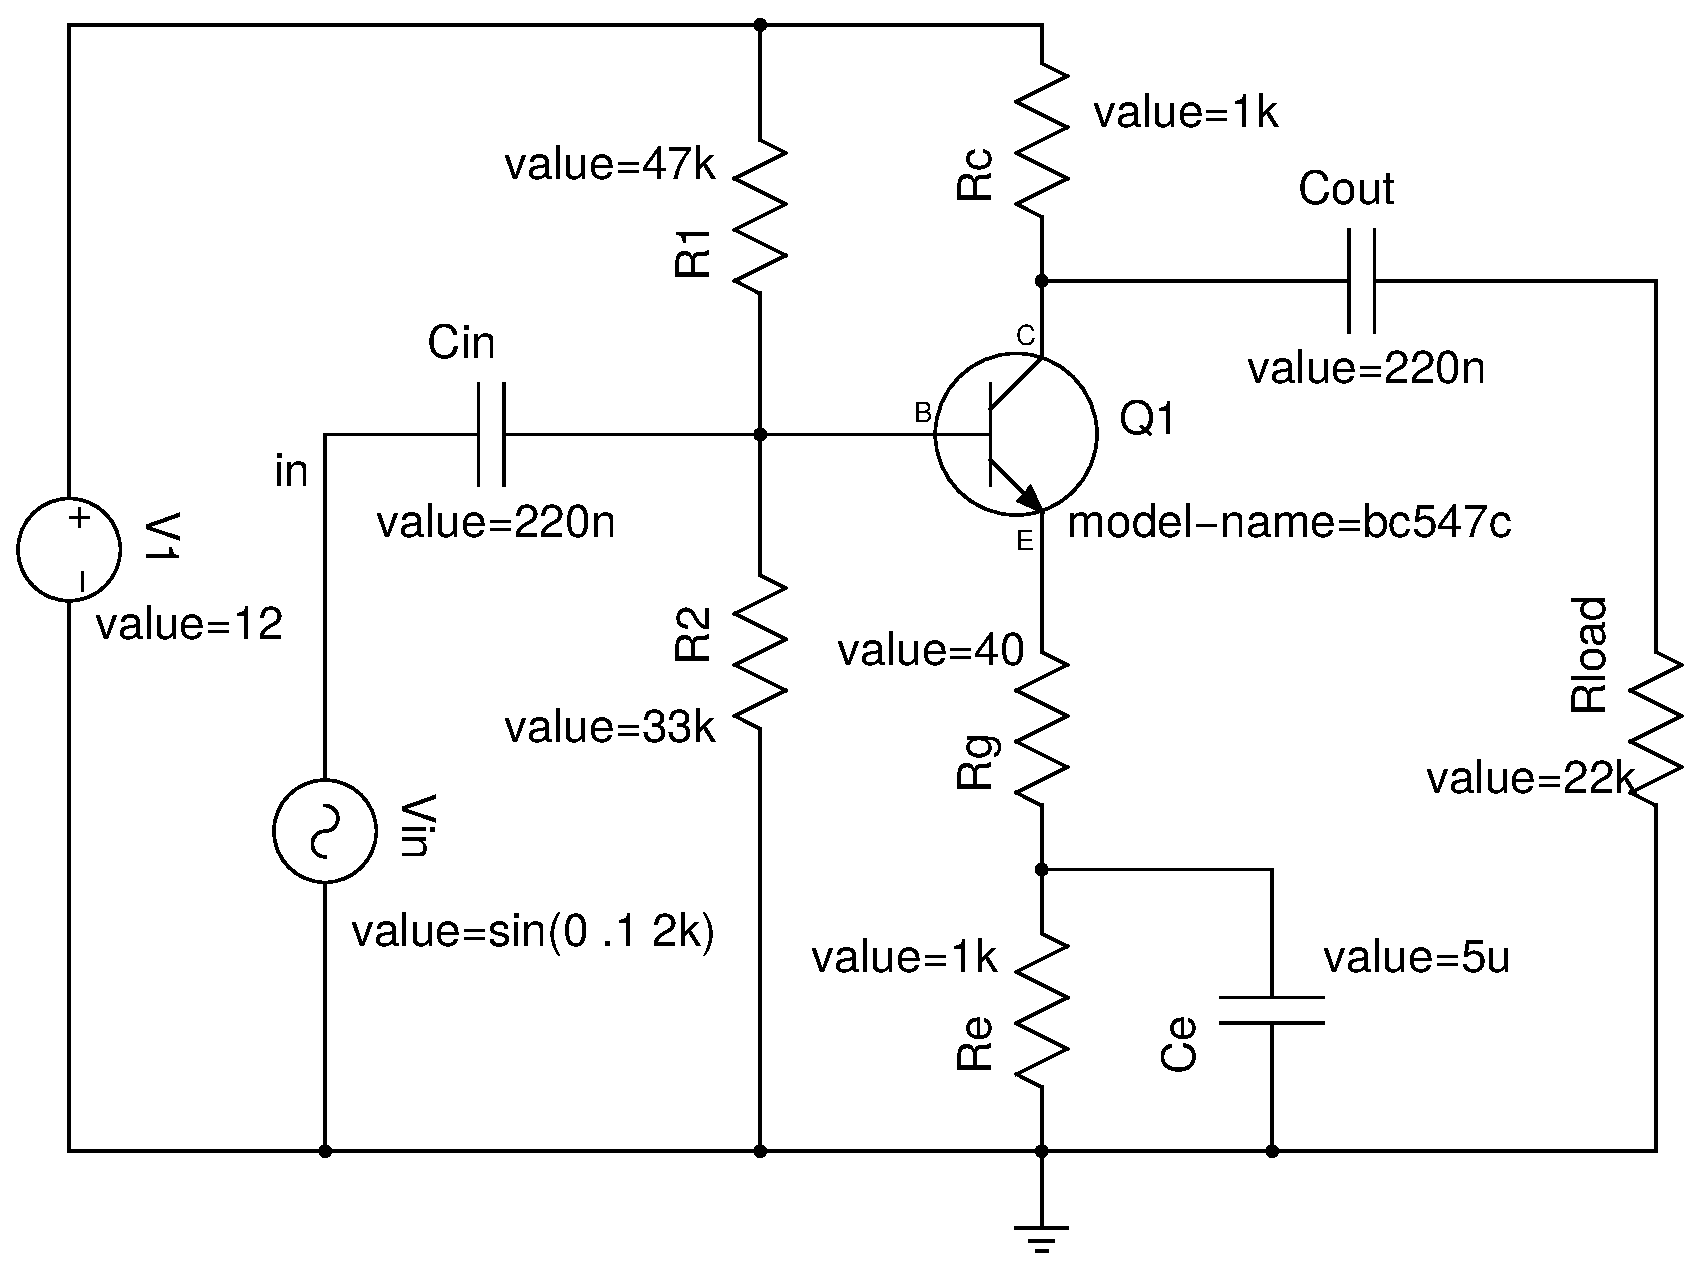
\includegraphics[scale=0.35]{ce-amplifier}
    \label{ce-amplifier}
    \caption{Circuit diagram for the common emitter amplifier}
\end{figure}

Resistors $R1$ and $R2$ are used to bias transistor $Q1$ in order to set the quiescent point of the transistor to the middle of its DC load line so that the collector of $Q1$ is put at $1/2$ of the supply voltage $V1$. This allows the maximum symmetrical swings of the output signal without clipping (flattening of the top or the bottom of the waveform). The collector voltage depends on the collector current (quiescent current), equation \ref{collector-voltage}. This current depends on the applied base bias and the values of $Rc$ and $Re$.

\begin{equation} \label{collector-voltage}
    V_c = V1 - I_c \cdot Rc
\end{equation}

Instead of using a voltage divider for biasing, it is possible to use only resistor $R1$, but this approach would make the quiescent point highly dependent on the current gain $\beta$ of the transistor. This parameter varies considerably in every transistor and the manufacturer usually specifies only a certain range of $\beta$. For this reason, we use a voltage divider constituted by $R1$ and $R2$ which impedance should be small compared with the impedance looking into the transistor base, formula \ref{divider-impedance}. This will give us a divider which is stiff enough so that the quiescent point is insensitive to variations in transistor $\beta$. However, the current flowing in the divider should not be unnecessarily large as it affects the overall consumption of the amplifier.

\begin{equation} \label{divider-impedance}
    R1 \| R2 \ll \beta Re
\end{equation}

Capacitors $Cin$ and $Cout$ form high pass filters and they are used as coupling capacitors to separate the AC signals from the DC voltage used to set up the amplifier. Their values are chosen so that the capacitors have low impedance for the desired input and output signal frequencies. This ensures that the signal's average is zero, as the capacitors pass only AC signals and block any DC component.

The input voltage $Vin$ causes a wiggle in the base voltage. The emitter voltage follows the base voltage which causes a wiggle in the emitter and also collector current. The output voltage which is the collector voltage depends on the current flowing through $Rc$, equation \ref{collector-voltage}. When this current rises, the collector voltage drops and vice versa. That means that the amplifier also inverts the input signal, figure \ref{ce-amplifier-sim}. The output AC signal is then superimposed on the collector DC voltage and the DC component is subsequently filtered out by the capacitor $Cout$ (high pass filter).

Capacitor $Ce$ is used to reach the amplifier's maximum gain. The values of $Re$ and $Rg$ set the emitter voltage which affects the amplifier's gain and we usually want these values to be as low as possible since this gives us the highest gain. However, if the emitter voltage is too low, it will vary significantly as the base-emitter drop varies with temperature. The solution is to bypass the $Re$ resistor so that the impedance for the emitter will vary according to the signal's frequency. The bypass capacitor $Ce$ is an open circuit component for DC bias and the emitter voltage depends on both $Re$ and $Rg$ which allows stable biasing. For higher frequency signals, the bypass capacitor short circuits $Re$ and the emitter voltage now depends mostly on $Re$ which value sets the maximum gain.

The analytical calculation for this circuit is beyond the scope of this thesis and it is left up to the evolutionary algorithms. The subject of the optimization are elements $R1$, $R2$, $Re$, $Rg$, $Rc$, $Cin$, $Ce$ and $Cout$. These elements represent the solution variables in the evolution strategies and make up the vector $\vec{x}$ which is thoroughly discussed in section \ref{mutation-section}. In this case, we optimize 8 components in the circuit so the search space has 8 dimensions.

\section{Two stage amplifier}
We can see the circuit diagram for a two stage amplifier on figure \ref{ce-amplifier-2stage}. The functionality and structure of the circuit are similar to the previous one with the difference that now we use two transistors connected in a cascade where transistor $Q1$ sends its output to the base of transistor $Q2$. This circuit was chosen as a more difficult problem to optimize, since the structure is twice as complicated as in the previous amplifier. The subject of the optimization are all the resistors and capacitors in the diagram apart from resistor $Rload$, so we have 14 compontents to optimize which makes the search space 14-dimensional.

\begin{figure}[H]
    \centering
    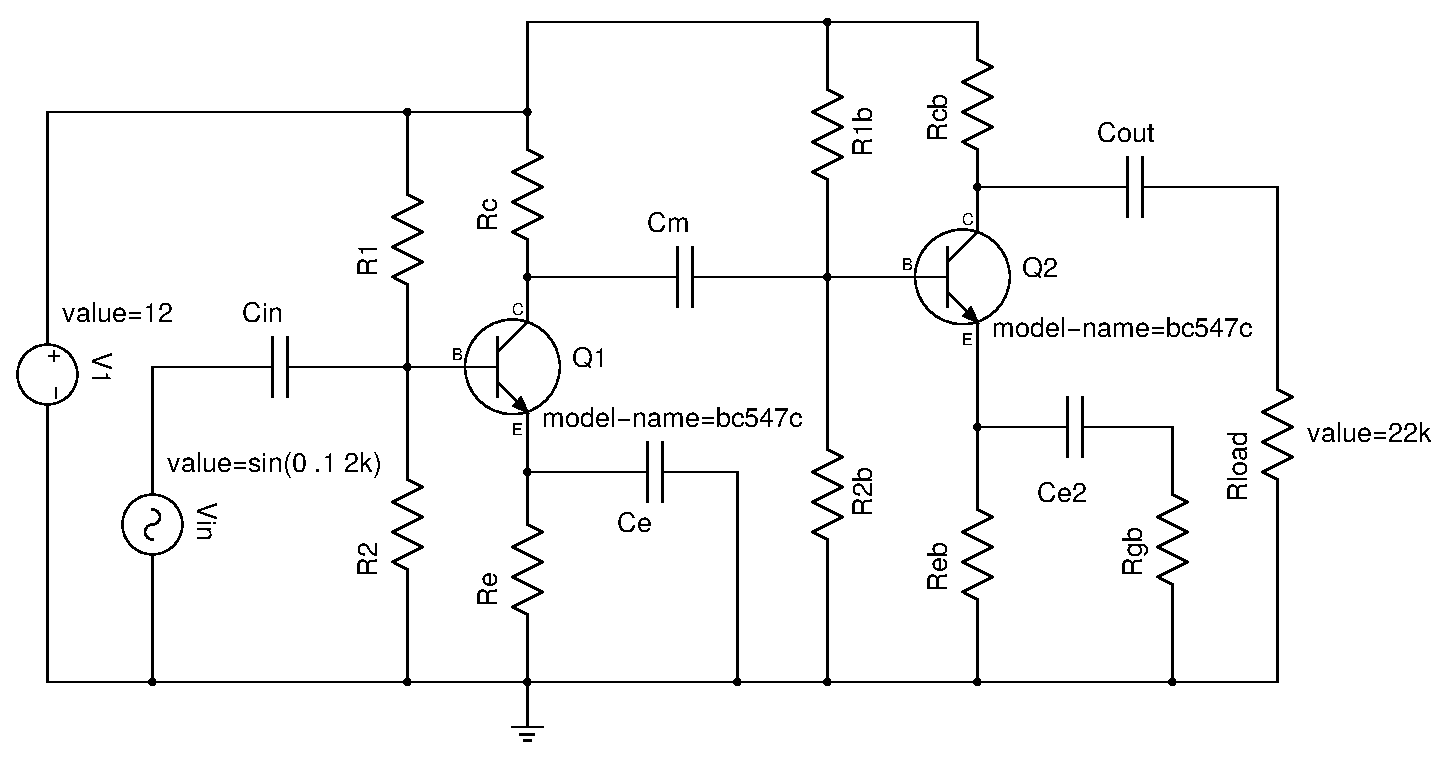
\includegraphics[scale=0.65]{ce-amplifier-2stage} \label{ce-amplifier-2stage}
    \caption{Circuit diagram for the two stage common emitter amplifier}
\end{figure}

\section{ngSPICE}
ngSPICE \footnote{ngSPICE home page - \url{http://ngspice.sourceforge.net/}} is an open-source, general-purpose circuit simulation program based on SPICE (\textit{Simulation Program with Integrated Circuit Emphasis}). It can simulate circuits with linear components and also nonlinear circuits which contain common semiconductor devices. Besides the simulation of analog circuits, it also offers simulation of digital circuits, in which case the simulator operates only with the logic states of the circuit, which has a great influence on the speed of the simulator. ngSPICE also offers a mixed-mode simulation where both the digital and analog simulations are combined together \cite{ngSPICE-manual}.

ngSPICE uses a language which syntax has been inherited from SPICE for describing circuits. An example of such description of the circuit from figure \ref{ce-amplifier} is shown in listing \ref{ce-amp-lst}. The first line contains the name of the circuit and on the next four lines, there is a description of the transistor used in the circuit. On the next lines, there is a list of the circuit's components. The name of the component is on the first position followed by the numbers or names of the nodes which the component is connected to. The last position contains the properties of the component. The second last line contains the description of the simulation. In this case, we do a transient analysis of the circuit for \SI{1.22}{\milli\second} with the sampling period \SI{20}{\micro\second} which provides us the time course of the amplifier's output signal. Later on, we use this data to evaluate the amplifier's quality.

Such netlist can be generated by using the gEDA \footnote{gEDA home page - \url{http://geda-project.org/}} (\textit{Electronic Design Automation}) toolkit which is also an open-source project oriented towards electronic design.

\begin{lstlisting}[caption={description of the common emitter amplifier using the SPICE syntax},
    label={ce-amp-lst},
    captionpos=b,
    numbers=left]
 amplifier
.model bc547c NPN (BF=730 NE=1.4 ISE=29.5F IKF=80M IS=60F
       + VAF=25 ikr=12m BR=10 NC=2 VAR=10 RB=280 RE=1 RC=40
       + VJE=.48 tr=.3u tf=.5n cje=12p vje=.48 mje=.5
       + cjc=6p vjc=.7 mjc=.33 isc=47.6p kf=2f)
Vin in 0 sin(0 .1 2k)
V1 4 0 9
Ce 0 5 5u
Cout 1 out 220n
Cin in 3 220n
Rc 1 4 1k
Rload 0 out 22k
Re 0 5 1k
Rg 5 2 40
R2 0 3 33k
R1 3 4 47k
Q1 1 3 2 bc547c
.TRAN 20u 1.22m
.end
\end{lstlisting}

In figure \ref{ce-amplifier-sim} we can see the simulation output of the circuit from listing \ref{ce-amp-lst} which is the same circuit as in figure \ref{ce-amplifier}. This circuit was also built using real electronic components in order to verify the simulation results. The measurement results of the real circuit proved that the simulator works correctly for this circuit as the measured values corresponded to the simulation.

\begin{figure}[!ht]
    \centering
    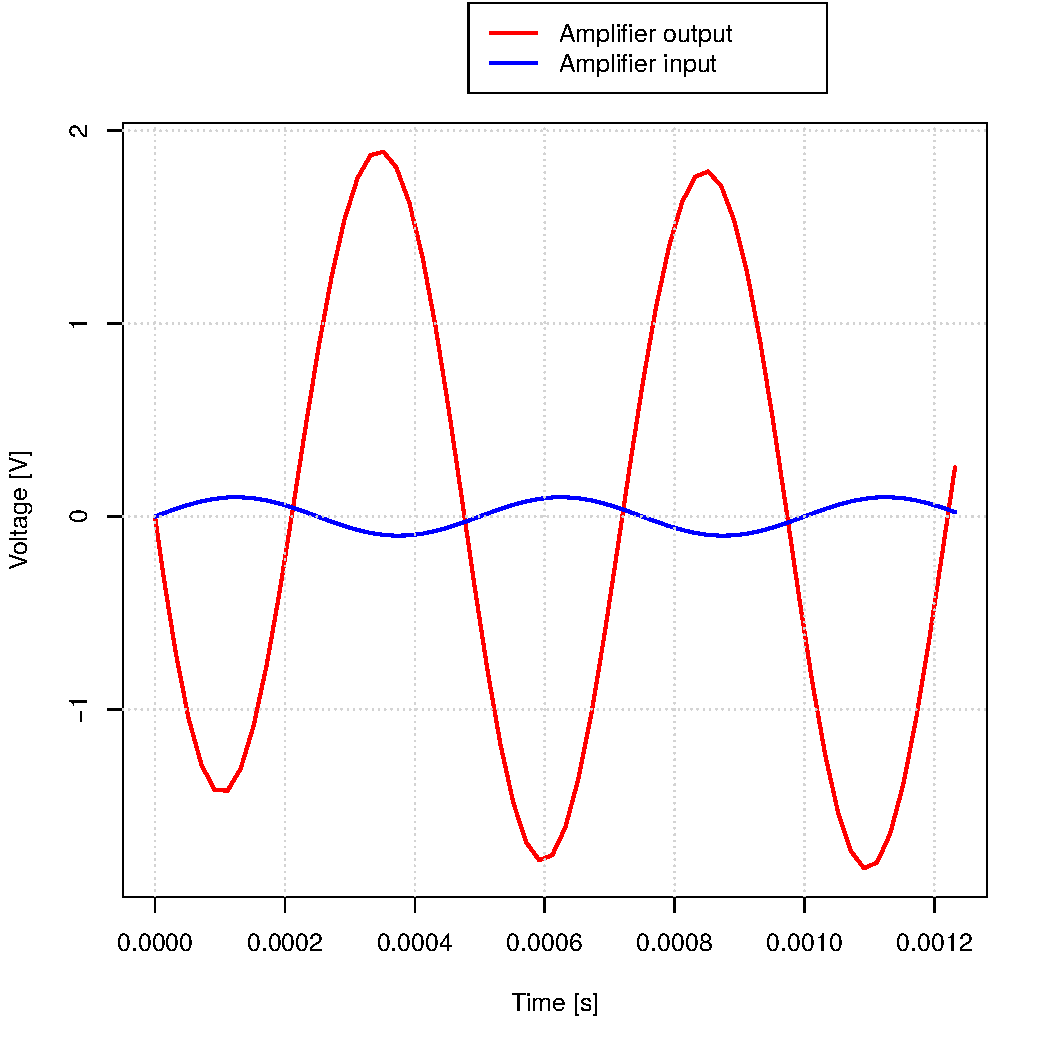
\includegraphics[scale=.6]{ce-amplifier-sim}\label{ce-amplifier-sim}
    \caption{Simulation of the common emitter amplifier}
\end{figure}

The last version of ngSPICE offers a C API which makes the simulator the ideal choice for utilizing it with the evolutionary algorithms. Every chromosome (candidate solution) in the evolution represents one amplifier and the simulator is used to determine the quality of it.

The API is used to pass the description of the amplifier to the simulator, run the simulation and obtain the simulation results. The results are in the form of arrays in C which represent time and the corresponding voltage values. These arrays have an equal length which depends on the simulation duration and the sampling period.

The default input frequency for the amplifier is \SI{2}{\kilo\hertz}, the duration of the simulation is set to \SI{1.22}{\milli\second} and it contains approximately two and a half period of the output signal. The duration does not need to be longer because the shape of the waveform does not change after the cicuit gets to a stable state. The sampling period is \SI{20}{\micro\second} so that the waveform is smooth enough on one hand and the simulation does not take too long on the other hand. The array containing the output voltage is used for the evaluation of the chromosomes which is thoroughly discussed in chapter \ref{chromosomes-evaluation}.

The simulator is launched several thousand times during a typical evolution and it takes most of the computation time. During the implementation of the algorithms discussed in section \ref{evolution-strategies} and the integration of the simulator, it emerged that there are memory leaks on several places in the source code of the simulator. This was a problem as the simulator leaked memory in every iteration. A significant amount of time was spent on fixing these bugs and the result is that the memory leaks have been removed. These improvements were proposed as a patch to the development team and they will be incorporated into the next versions of ngSPICE.

\chapter{Evaluation of amplifiers} \label{chromosomes-evaluation}
A fitness function provides the means to determine how good the evolved solution is so that the most appropriate candidates can be distinguished from the less appropriate ones. It is important to mention that the quality of this function is essential because the ability of the algorithm to find the most suitable solution is highly dependent on the ability of the fitness function to distinguish between the individuals. The value of the function is a positive real number in our case and the algorithm uses it only for comparing the individuals between each other. We consider those individuals with the lower value as the better ones.

The implementation required some methods of trial and error and in the end, there are three fitness functions implemented in this thesis. All of them use the ngSPICE simulator in order to obtain the output of the amplifier and assess it afterwards. The simulation is done for every candidate solution and it takes most of the computation time of the overall evolutionary algorithm.

\section{Best match with the reference solution}
This fitness function has been implemented as the first one in order to find out if the evolution has at least the ability to get close to the analytical solution. It is based on the method of least squares which is used in regression analysis.

The fitness function uses the output voltage vector from the simulator for assessing the chromosomes. The vector represents the waveform of the output signal from the circuit and the shape of the waveform gets similar to an inverted sine wave as the solution evolves. The length of the vector is set to 69 (the sampling period is approximately \SI{20}{\micro\second}) elements during the whole evolution and the vector contains approximately 2.5 periods of the signal (the signal's frequency is \SI{20}{\kilo\hertz}). The fitness function uses two types of these vectors, one serves as the reference vector (the output of the amplifier which elements' values were calculated analytically) and all the candidate vectors are compared to it. As we can see in figure \ref{ce-amplifier-sim}, the first period of the signal is unstable, so the fitness function skips it and picks only the second period for comparison with the reference signal. It is sufficient to compare only the second period because the shape of the signal doesn't change anymore after the circuit gets to a stable state.

The functions in algorithm \ref{get-second-period} are used to extract the second period from the waveform. Since the vector has a constant length and the values represent an inverted sine wave, we can walk through the first two and the last half-period to get to the desired part of the signal.

The first function starts at the start of the vector and it skips the first half-period which values are less than zero and it also skips the second half-period in a similar way. The second function starts from the end of the vector and it skips the second last period of the signal in the vector. The resulting $start$ and $end$ indices point to the start and the end of the second period of the signal.

When the evolution starts, the waveform of some candidate solutions is not in the shape of an inverted sine wave and therefore it crosses zero sooner than the desired waveform. In this case, the algorithm ends with indices close to the starting and ending index and such candidate solution is assessed with a high fitness value.

    \begin{algorithm}
    \caption{Find the first and last index of the second period}
    \label{get-second-period}
    \begin{algorithmic}[1]
        \Function{getStart}{$vector$}
            \State $start \gets 0$;
            \While{$vector[start] < 0$}
                \State $start \gets start + 1$;
            \EndWhile
            \While{$vector[start] > 0$}
                \State $start \gets start + 1$;
            \EndWhile
            \State \Return $start$;
        \EndFunction
        \State

        \Function{getEnd}{$vector$}
            \State $end \gets vector.length()$;
            \While{$vector[end] < 0$}
                \State $end \gets end - 1$;
            \EndWhile
            \State \Return $end$;
        \EndFunction
    \end{algorithmic}
    \end{algorithm}

The function in algorithm \ref{bestFit} is used to evaluate the candidate solutions. It iterates over the second period in both reference and candidate vectors and it calculates the sum of squares which sides are defined by the difference between the values in the reference vector and the candidate vector. The overall sum is returned as the result of the fitness function and the lower the value, the better the candidate solution is.

The reason why we add up squares and not only the absolute values of the differences is important. Consider two imaginary vectors of two values which differ from the reference vector by $(1, 5)$ and by $(3,3)$. The sum of the absolute values is 6 in both cases, so this method doesn't distinguish between these vectors. However, the sum of the squares is 26 for the first vector and 18 for the second one. This difference is important as we want all the values to be close to the reference and not only some of them and therefore the second vector is assessed as the better one.

\begin{algorithm}
\caption{Fitness evaluation using the analytical solution}
\label{bestFit}
\begin{algorithmic}[1]
    \Function{rateChromosome}{$candidateVector$, $referenceVector$}
        \State $fitness \gets 0$;
        \State $start \gets$ \Call{getStart}{$candidateVector$};
        \State $end \gets$ \Call{getEnd}{$candidateVector$};
        \For{$i \gets start : end$}
            \State $fitness \gets fitness + (referenceVector[i] - candidateVector[i])^2$;
        \EndFor
        \State \Return $fitness$;
     \EndFunction
\end{algorithmic}
\end{algorithm}

We can see the result of the evolution using this fitness function in figure \ref{best-match}.

\begin{figure}[H]
    \centerline{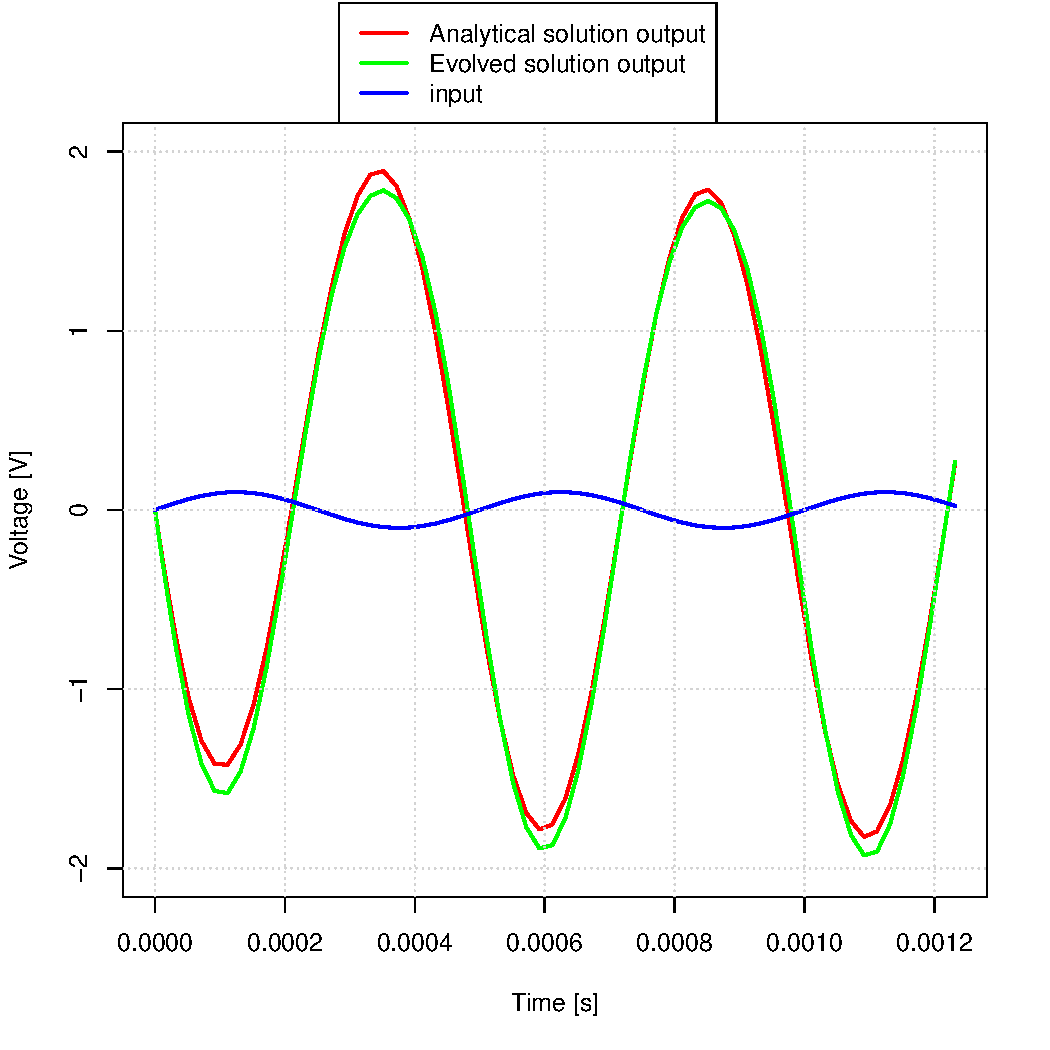
\includegraphics[scale=0.6]{best-match}\label{best-match}}
    \caption{The result of evolution towards the analytical solution}
\end{figure}

\section{Ideal sine wave}
This method is similar to the previous one but instead of using the pre-simulated output as a reference, it uses an analytically calculated sine wave. An analytical sine wave is used in order to force the evolution towards such solution that won't produce a distorted output signal since the input is in the form of a sine wave as well. The function also uses the method of least squares explained in the previous section and it iterates over the second period of the signal which is represented by the $candidateVector$.

We can see the technique in algorithm \ref{idealSine}. In every iteration, it calculates the value of the sine wave and compares it with the simulated signal. The sum of the comparisons is then returned as the fitness value and the lower the result is, the closer the candidate solution is to the reference. The amplitude of the sine wave is set by the user, so this method allows users to design amplifiers with an arbitrary amplification which doesn't exceed the circuit's capabilities.

\begin{algorithm}[H]
\caption{Fitness evaluation using the ideal sine wave}
\label{idealSine}
\begin{algorithmic}[1]
    \Function{rateChromosome}{$candidateVector$, $amplitude$}
        \State $fitness \gets 0$;
        \State $start \gets$ \Call{getStart}{$candidateVector$};
        \State $end \gets$ \Call{getEnd}{$candidateVector$};
        \State $refSineSize \gets end - start$;
        \For{$i \gets 0 : refSineSize$}
           \State \scalebox{1.3}{$refSine \gets -amplitude \cdot \sin(\frac{2 \pi i}{refSineSize - 1})$};
           \State $fitness \gets fitness + (refSine - candidateVector[start + i])^2$;
        \EndFor
        \State \Return $fitness$;
    \EndFunction
\end{algorithmic}
\end{algorithm}

\section{Maximal amplitude}
This fitness function is designed to rate the candidate solutions only according to the amplitude of the output regardless of the waveform's shape. It can be used for finding the highest amplification capabilities of the circuit. The function finds the trough and the peak in the second period and returns the multiplicative inverse of their difference.

\begin{algorithm}[H]
\caption{Rating the chromosomes according to the amplitude}
\label{maxAmp}
\begin{algorithmic}[1]
    \Function{rateChromosome}{$candidateVector$}
        \State $start \gets$ \Call{getStart}{$candidateVector$};
        \State $end \gets$ \Call{getEnd}{$candidateVector$};
        \State $trough \gets \min(candidateVector[start]$, $candidateVector[end])$;
        \State $peak \gets \max(candidateVector[start]$, $candidateVector[end])$;
        \State \Return \scalebox{1.2}{$\frac{1}{peak - trough}$};
    \EndFunction
\end{algorithmic}
\end{algorithm}

\section{Waveform symmetry}
All of the fitness functions discussed above have difficulties in finding symmetrical waveforms. An example is shown in figure \ref{asymmetrical-ideal-sine}.

\begin{figure}[!ht]
    \centerline{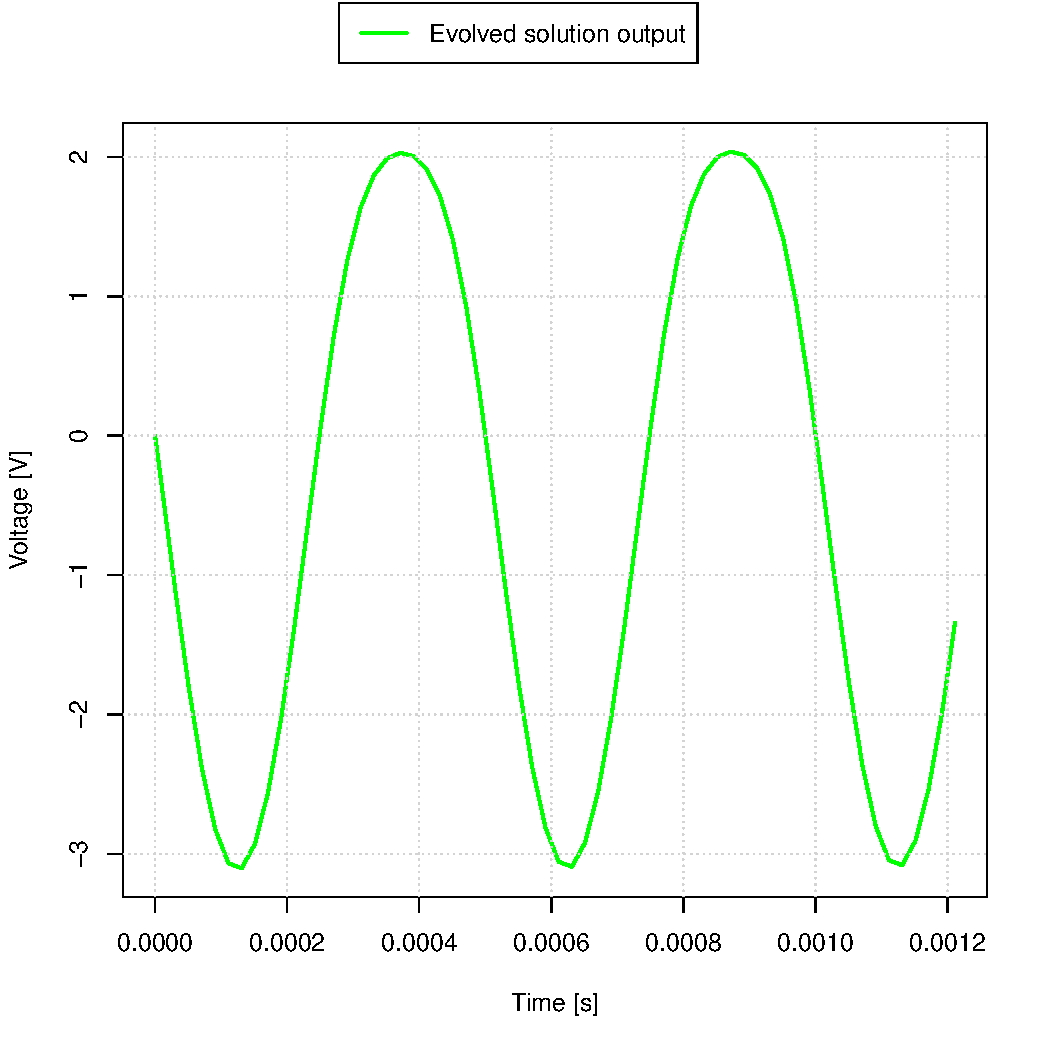
\includegraphics[scale=0.6]{asymmetrical-ideal-sine}\label{asymmetrical-ideal-sine}}
    \caption{An asymmetrical result of the evolution using the 'ideal sine wave' evaluation}
\end{figure}

The problem is that at the start, the output signal has zero power and as the evolution continues, only one half of the signal rises and the fitness function value decreases even though the evolution doesn't go in the right direction. At the end, the evolution ends up in the state shown in figure \ref{asymmetrical-ideal-sine}. The first solution to this problem is described in formula \ref{sym1}.

\begin{equation} \label{sym1}
result = (|peak + trough| + 1) \cdot fitness
\end{equation}

The $peak$ and $trough$ values are obtained in the same way as in algorithm \ref{maxAmp}. If the signal is symmetrical, the absolute value of the sum of these values is close to zero and therefore the $result$ will also be lower. We add 1 to the sum because we need to distinguish between perfectly symmetrical signals with different fitness. However, it emerged that this approach is too restrictive as it promotes only signals which are perfectly symmetrical, but often distorted. The result is shown in figure \ref{symmetrical-ideal-sine}.

\begin{figure}[!ht]
    \centerline{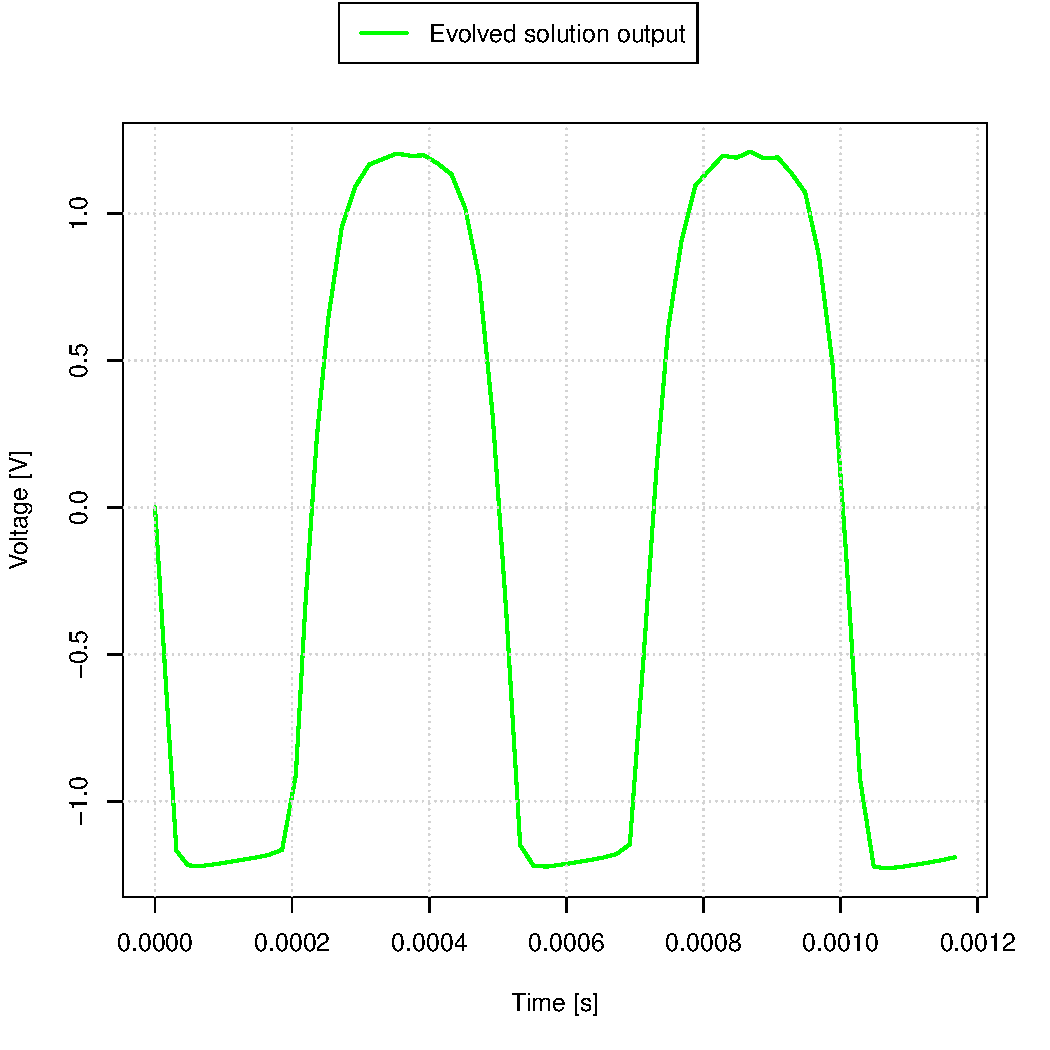
\includegraphics[scale=0.6]{symmetrical-ideal-sine}\label{symmetrical-ideal-sine}}
    \caption{A distorted result using the 'ideal sine wave' evaluation with perfect symmetry}
\end{figure}

The ability of the evolution to find the desired solution was also decreased because some asymmetrical candidate solutions head towards a good solution. These consequences led to another solution to this problem.

\begin{algorithm}
\caption{Rating the chromosomes with regard to the symmetry of the signal}
\label{symmetry-rating}
\begin{algorithmic}[1]
    \Function{rateChromosome}{$candidateVector$, $maxDifference$}
    \State $min \gets \min(|trough|$, $peak)$;
    \State $max \gets \max(|trough|$, $peak)$;
    \If{\scalebox{1.1}{$\frac{min}{max} < (1 - \frac{maxDifference}{100})$}}
        \State \Return $DOUBLE\_MAX$;
    \EndIf
    \LineComment{continue evaluating the chromosome}
    \EndFunction
\end{algorithmic}
\end{algorithm}

Condition on line 4 in algorithm \ref{symmetry-rating} is used to separate the symmetrical and asymmetrical chromosomes. The values of the variables $trough$ and $peak$ are obtained in the same way as in algorithm \ref{maxAmp}. The value of $maxDifference$ is in the interval $\left]0, 100\right]$ and it is set by the user. It represents the maximal percentage difference between the peak and trough in the second period of the signal. The algorithm calculates the ratio between the peak and trough and if the result is less than the threshold value, the chromosome is evaluated with the maximal fitness and the function is terminated. Otherwise, the evaluation continues. This allows the user to control the results of the evolution with respect to the symmetry of the output signal.

\chapter{Experiments}
The evolutionary algorithms described in section \ref{evolution-strategies} were implemented in C++. This language was chosen due to its flexibility, performance and the possibility to make use of the ngSPICE simulator. The implementation also utilizes the RInside \footnote{RInside home page - \url{http://dirk.eddelbuettel.com/code/rinside.html}} library which integrates R \footnote{R home page - \url{https://www.r-project.org/}} into C++ \cite{Rcpp}. The R language is used to plot graphs dynamically during the evolution either to the screen or to a file so the user can see and record how the solution evolves.

The program is written as a console application and the user can specify the properties of the evolution via command-line arguments. This approach also allows the user to easily run the application multiple times and collect the results of the evolution.

The results are in the form of graphs and a text output which contains the details about the evolution run. The graphs can be either dynamically generated to the screen during the program run or saved as files to the local drive as well as the text output. The user can specify how often the graphs and text description are generated, for example, each time the fitness function of the best chromosome in the population decreases by 1\%.

The results of the experiments discussed below are related to the evolutionary algorithm itself. The results of the optimization of the amplifiers are analyzed in sections \ref{single-stage-results} and \ref{2stage-results}.

\section{Initial stages of experiments}
The first experiments were performed only in order to optimize the value of resistor $R1$ in the single stage amplifier. The 'best match' evaluation method and mutations with one step size were used. The evolution always found a value close to \SI{50}{\kilo\ohm} which was the desired solution. These experiments were always successful as this was a very simple task for the evolution.

In the next stage, the task was to optimize the voltage divider constituted by $R1$ and $R2$. The 'best match' method and mutations with one step size were used again and it emerged, that the evolution was able to find the solution even faster than in the previous case. This was because we were looking only for the right ratio between the resistors and not for specific values so the set of the desired solutions was much larger in this case even though the search space was larger as well as it was two-dimensional.

The next task for the evolution was to find the right values for resistors $R1$, $R2$ and $Rg$. The evolution parameters were set in the same way as in the previous experiments. This task showed the weak spot of mutations with one step size as the evolution was able to find an acceptable solution very rarely. The reason was that the desired value of $Rg$ is very close to the lower bound of the search space (the analytical value is only \SI{40}{\ohm}). Since mutations with one step size use the same mutation value in every dimension, it was not possible to mutate $Rg$ only by a few ohms (not to move away from the lower bound of this dimension) and at the same time look for the right values in other dimensions which required steps in kiloohms. The value of $Rg$ heavily influences the overall fitness of the chromosome because high values significantly decrease the gain of the amplifier. The usual course of the evolution was that the value of $Rg$ converged quickly to the lower boundary and since this parameter has a great influence on the fitness, the evolution preferred chromosomes with this property. This led to a quick decrease of the mutation step size $\sigma$ (the fitness function also indirectly evaluates the value of $\sigma$) and the algorithm got stuck in a local optimum since other dimensions (values of other resistors) in the search space could not be searched properly. The solution to this problem was to implement mutations with $n$ step sizes discussed in section \ref{n-step}. This approach allows us to treat every dimension separately and therefore search the search space more effectively. After the implementation, the evolution was able to find a satisfactory solution in most of its runs.

The previous experiments proved that the evolutionary algorithms are able to provide acceptable solutions in the domain of analog amplifiers. The next section describes the process of determining the ideal parameters for the evolution.

\section{Evolution parameters}
In order to make the evolution strategies work efficiently, we need to find and set the correct parameters for the evolution.

The size of the search space is defined by the number of dimensions and by the size of every dimension. The number of dimensions depends on the number of electronic components that we want to optimize and the sizes of the dimensions depend on the range of the values that every component can have. These ranges were set from \SIrange{0}{200}{\kilo\ohm} for resistors and from \SIrange{0}{500}{\micro\farad} for capacitors. The upper bounds are based on the values of real electronic components so, for example, we do not expect to have a higher resistance than \SI{200}{\kilo\ohm} in the circuit. The values of some particular components could have a smaller range, for example, resistor $Rg$ which value does not need to be higher than a few kiloohms, but the assumption is that we have no knowledge about the circuit at all.

The initial mutation step size $\sigma$ is set to 100. This value is not very important because this parameter is adapted during the evolution. Experiments showed that there is no difference between setting the initial $\sigma$ to 10 or 500 for example. However, if we set the initial value too high (10000 and above), it is more likely that the evolution will get stuck in a local optimum because the algorithm converges too quickly at the start.

The experiments also showed that the values of the learning parameters $\tau$ and $\tau'$ have a significant impact on the speed at which the evolution converges to the optimum. The higher the values were, the faster the evolution converged, nevertheless this also means that the probability of finding only a local optimum was rapidly increased. For this reason, the values were set according to formulas \ref{set-tau} and \ref{set-tau-prime} to their lowest possible values. The parameter $n$ is the number of dimensions of the search space.

\begin{equation} \label{set-tau}
    \tau = \frac{1}{\sqrt{n}}
\end{equation}

\begin{equation} \label{set-tau-prime}
    \tau' = \frac{1}{\sqrt{2\sqrt{n}}}
\end{equation}

The maximum difference between the peak and trough of the amplifier's output waveform was empirically set to 25. This means that the values of the peak and trough of the waveform can differ at most by 25\%.

\section{Population size, selection type and selective pressure}
\label{population-size}
Important parameters of the evolution are numbers $\mu$ and $\lambda$ which define the population size (the number of parents and children in every generation) and the selective pressure which is defined by the ratio between $\mu$ and $\lambda$. The next important parameter is the type of the selection that we choose for the evolution (($\mu$, $\lambda$)-ES or ($\mu + \lambda$)-ES). In order to determine the most suitable values of the parameters, there were various experiments carried out which are summarized in table \ref{experiments-results}.

Every row of the table contains results for a different combination of $\mu$ and $\lambda$. The values of $\mu$ are set to 1, 5, 10 and 15 and the selective pressure is also 1, 5, 10 and 15 for every value of $\mu$, so there are four different values of $\lambda$ for every $\mu$. For every such combination, there are results for both selection types and under every type, there are three columns representing all the three evaluation methods that are discussed in chapter \ref{chromosomes-evaluation}. One cell of the table corresponds to the result of one experiment where the evolutionary algorithm was run 10 times with the same parameters and the fitness values of the resulting chromosomes were added up and divided by 10. The task was to optimize the single stage amplifier.

We can see that there is no significant difference between the selection schemes, provided the selective pressure is higher than one. On lines 5, 9 and 13 (where the selection pressure is 1) the ($\mu$, $\lambda$)-ES scheme performs significantly worse than the ($\mu + \lambda$)-ES scheme and even increasing the population size has no effect (line 5 compared to line 9 and 13). However, when we sum up all the values in both schemes (excluding lines 1, 5, 9 and 13), the latter one gives us better results, so the ($\mu + \lambda$)-ES selection scheme was chosen as the more effective one.

We can also see that when the value of $\mu$ is only 1, the algorithm's results are substantially worse than in the rest of the table and on the other hand when we increase it from 5 to 15, there is only a small change in the overall performance.

The value of $\lambda$ is set according to the value of $\mu$ multiplied by the selection pressure and it highly influences the overall computation time of the algorithm because it defines the number of chromosomes that have to be evaluated in every generation (the evaluation includes the amplifier's simulation which takes most of the computation time). When the selective pressure and the value of $\mu$ are higher than one, the overall efficiency of the algorithm does not increase rapidly but there is a noticeable increase in the computation time. For this reason, the values of $\mu$ and $\lambda$ were set to $\mu = 15$ and $\lambda = 150$ as a compromise between the algorithm's time demands and the optimization efficiency. Higher values were also examined but they did not provide any significant improvements.

\begin{table}[H]
\centering
\begin{tabular}{@{}ccccccccc@{}}
\toprule
    &       &           & \multicolumn{3}{c}{($\mu$, $\lambda$)-ES} & \multicolumn{3}{c}{($\mu + \lambda$)-ES} \\
   \cmidrule(lr){4-6} \cmidrule(lr){7-9}
    & $\mu$ & $\lambda$ & best match & ideal sin & max. ampl.       & best match & ideal sin  & max. ampl.     \\
   \midrule
1.  & 1     & 1         & N/A        & N/A       & N/A              & 21.82      & 99.00      & 2.90           \\
2.  & 1     & 5         & 20.82      & 113.75    & 1.98             & 13.44      & 57.91      & 2.69           \\
3.  & 1     & 10        & 18.84      & 76.81     & 1.40             & 24.70      & 75.01      & 2.84           \\
4.  & 1     & 15        & 18.43      & 128.75    & 2.26             & 19.52      & 34.11      & 1.02           \\
5.  & 5     & 5         & 49.62      & 169.02    & 36.50            & 9.81       & 56.61      & 3.18           \\
6.  & 5     & 25        & 7.28       & 55.00     & 3.12             & 12.12      & 34.88      & 2.72           \\
7.  & 5     & 50        & 16.18      & 64.22     & 3.21             & 9.75       & 43.73      & 3.57           \\
8.  & 5     & 75        & 3.70       & 58.82     & 3.10             & 4.20       & 38.84      & 3.52           \\
9.  & 10    & 10        & 49.41      & 154.66    & 26.40            & 8.94       & 53.77      & 3.18           \\
10. & 10    & 50        & 9.09       & 60.93     & 2.68             & 7.02       & 45.04      & 3.58           \\
11. & 10    & 100       & 6.97       & 38.02     & 3.16             & 4.91       & 26.06      & 3.10           \\
12. & 10    & 150       & 8.06       & 25.54     & 3.10             & 2.52       & 23.07      & 3.07           \\
13. & 15    & 15        & 44.48      & 165.76    & 34.99            & 2.54       & 47.69      & 3.18           \\
14. & 15    & 75        & 4.64       & 56.18     & 2.25             & 4.96       & 51.74      & 3.56           \\
15. & 15    & 150       & 6.63       & 47.32     & 3.52             & 6.36       & 12.19      & 1.60           \\
16. & 15    & 225       & 7.56       & 31.17     & 2.65             & 0.70       & 19.31      & 1.08           \\
    \bottomrule
\end{tabular}
\caption{Results of experiments, cells contain results where the evolution was run 10 times and the fitness values of the resulting chromosomes were added up and divided by 10}
\label{experiments-results}
\end{table}


All the evolution parameters discussed above are summarized in table \ref{evolution-parameters}. These parameters were chosen as the most appropriate ones.

\begin{table}[H]
\centering
\begin{tabular}{@{}ll@{}}
\toprule
    Parameter                   & Value \\ \midrule
    Resistance range            & \SIrange{0}{200}{\kilo\ohm} \\
    Capacitance range           & \SIrange{0}{500}{\micro\farad} \\
    initial $\sigma$            & 100 \\
    max. peak-trough difference & 25 \% \\
    $\mu$                       & 15 \\
    $\lambda$                   & 150 \\
    selection type              & ($\mu + \lambda$)-ES \\
    $\tau$                      & equation \ref{set-tau}\\
    $\tau'$                     & equation \ref{set-tau-prime} \\ \bottomrule
\end{tabular}
\caption{Optimal evolution parameters}
\label{evolution-parameters}
\end{table}

\section{The typical course of the evolution}
Figure \ref{evolution-course} shows the typical course of the evolution. The population size parameters were set to $\mu = 10$ and $\lambda = 100$ and the terminating condition of the algorithm was that the evolution ends when the value of the fitness function of the best chromosome does not decrease by more than 1\% after 300 generations.

The green line represents the fitness of the best chromosome (the one with the lowest fitness) in every generation, the blue line is the fitness of the worst chromosome and the red line is the average fitness of every generation. In this case, we pick the chromosomes only from the set of $\mu$ parents. We can see that the red line is very close to the green line so the average fitness of every generation is close to the fitness of the best chromosome and that the blue line is scattered above the other two lines.

The evolution was stuck in a local optimum for approximately 20 generations between the 80th and 100th generation and the solution was evolved approximately after 300 generations. When the blue line is close the other two lines, it means that the sizes of the mutation steps $\sigma$ are low and the algorithm searches only a small area of the search space. When the values of $\sigma$ are low (close to zero), we can stop the algorithm after a few hundreds of generations because it will not provide any better solution than the current one and the resulting fitness is either in a local or global optimum.

The amount of generations needed for the optimization is usually a few hundred, as also shown in figure \ref{evolution-course}. When the size of the population is low (for example $\mu = 1$ and $\lambda = 5$), the optimization takes a few thousands of generations. In any case, there is approximately up to 30000 simulations in every evolution run which takes a few minutes (usually between two to four minutes) on the Intel Core i5-5200U processor.

In this case, the evaluation method was the 'best match' method and this evolution run was successful since the resulting fitness was very close to zero. With this method, we can consider those solutions which fitness is under 0.5 as sufficient because the amplifier's output waveform is very close to the desired one. The resulting value of the fitness of the best chromosome was 0.19.

\begin{figure}[H]
    \centerline{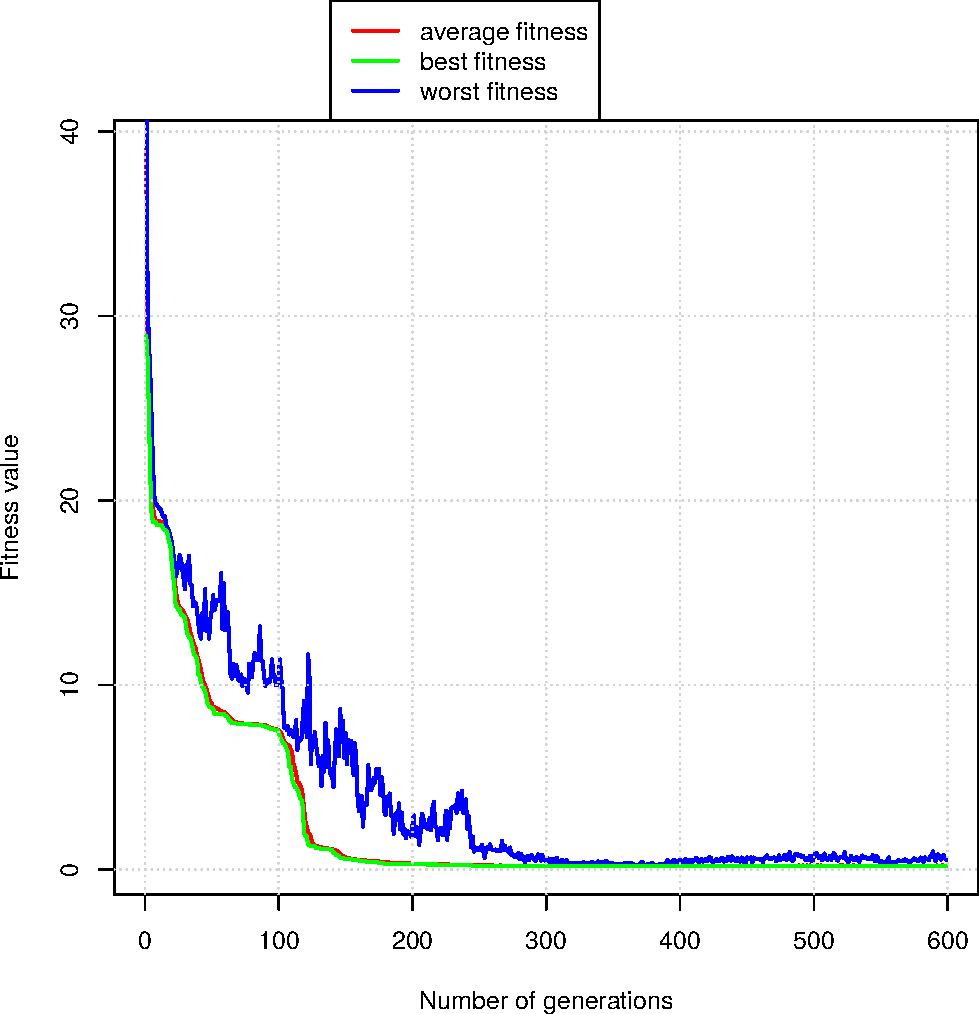
\includegraphics[scale=0.6]{evolution-course}
    \label{evolution-course}}
    \caption{The typical course of the evolution}
\end{figure}

\section{Single stage amplifier optimization} \label{single-stage-results}
Every evaluation method implemented in this thesis provides different means by which we can optimize the circuit.

The 'best match' method can be used for finding such properties that provide the most similar output compared to the analytical solution. We optimize the values of 8 electronic components and experiments with this method proved that there are many other possible combinations which provide almost identical behaviour of the amplifier. Five examples are shown in table \ref{best-fit-solutions}. The simulation output of the amplifier with these values of components was visually identical with the analytical solution.


\begin{table}[H]
\centering
\begin{tabular}{@{}c ccccccc@{}}
\toprule
    $R1$ [\si{\kilo\ohm}] & $R2$ [\si{\kilo\ohm}] & $Re$ [\si{\ohm}] & $Rg$ [\si{\ohm}] & $Rc$ [\si{\kilo\ohm}] & $Ce$ [\si{\nano\farad}] & $Cin$ [\si{\nano\farad}] & $Cout$ [\si{\nano\farad}] \\
    \midrule
    200   & 76.2 & 7510  & 471 & 21.7 & 460     & 29    & 1010 \\
    78.5  & 16   & 3370  & 429 & 23   & 228 000 & 17    & 396 000 \\
    141   & 11.5 & 180   & 483 & 21.1 & 285 000 & 21    & 280 000 \\
    82.3  & 44.3 & 8590  & 400 & 16   & 499     & 202   & 95 \\
    118   & 41.2 & 11500 & 559 & 35.4 & 419     & 95    & 19 \\
    \bottomrule
\end{tabular}
\caption{Values of components that provide visually identical outputs with the analytical solution}
\label{best-fit-solutions}
\end{table}

The 'maximal amplitude' method can be used for finding the best amplification capabilities of the circuit as it does not take into consideration the shape of the output signal. This method is useful for the 'ideal sine' method because it allows us to find the appropriate maximal amplitude and then we can find the right waveform by using the latter method. By this approach, we can find even better solutions than the analytical one. One of such solutions is shown in figure \ref{better-solution-fig} and the values of the components are summarized in table \ref{better-solution-tab}. Since the amplitude of the input signal was $Vin = \SI{100}{\milli\volt}$ and the amplitude of the output signal is approximately \SI{4.2}{\volt}, the gain of this amplifier is approximately 42 (the gain of the analytically solved amplifier is approximately 18). The gain also depends on the voltage $V1$ that supplies the amplifier which is set to $V1 = \SI{12}{\volt}$ in the experiments.

\begin{figure}[!htb]
    \centerline{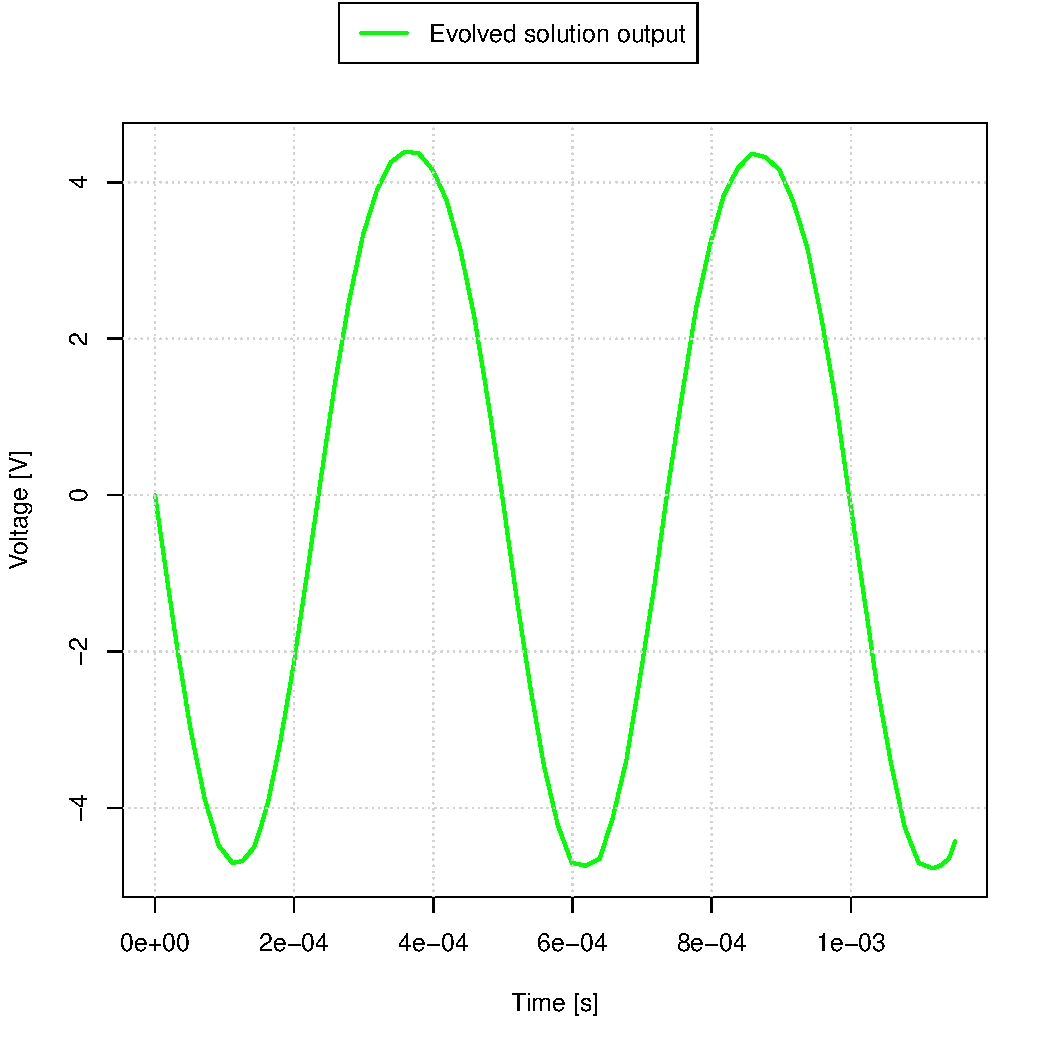
\includegraphics[scale=0.6]{best-solution-single-stage}\label{better-solution-fig}}
    \caption{The best solution for the single stage amplifier found by the evolution}
\end{figure}

\begin{table}[H]
\centering
\begin{tabular}{@{}cccccccc@{}}
\toprule
    $R1$ [\si{\kilo\ohm}] & $R2$ [\si{\kilo\ohm}] & $Re$ [\si{\ohm}] & $Rg$ [\si{\ohm}] & $Rc$ [\si{\kilo\ohm}] & $Ce$ [\si{\micro\farad}] & $Cin$ [\si{\micro\farad}] & $Cout$ [\si{\nano\farad}] \\
    \midrule
    168 & 15.1 & 169 & 49 & 4.21 & 16 & 274 & 86 \\
    \bottomrule
\end{tabular}
\caption{The best solution for the single stage amplifier found by the evolution}
\label{better-solution-tab}
\end{table}

The 'ideal sine' evaluation method also provides a universal tool for finding the appropriate values of components which produce an arbitrary amplification of the amplifier up to the maximal amplitude.

\section{Two stage amplifier optimization} \label{2stage-results}
This amplifier was chosen as the more complicated task to optimize. There was no analytical solution for this circuit so it was not possible to use the 'best match' evaluation method. Experimenting with this type of amplifier showed that this amplifier is much more difficult to optimize and that it does not provide any better amplification properties than the previous single stage amplifier.

The same set of experiments was carried out as for the previous amplifier and one of the best solutions is shown in figure \ref{best-solution-two-stage-fig}.

\begin{figure}[ht]
    \centerline{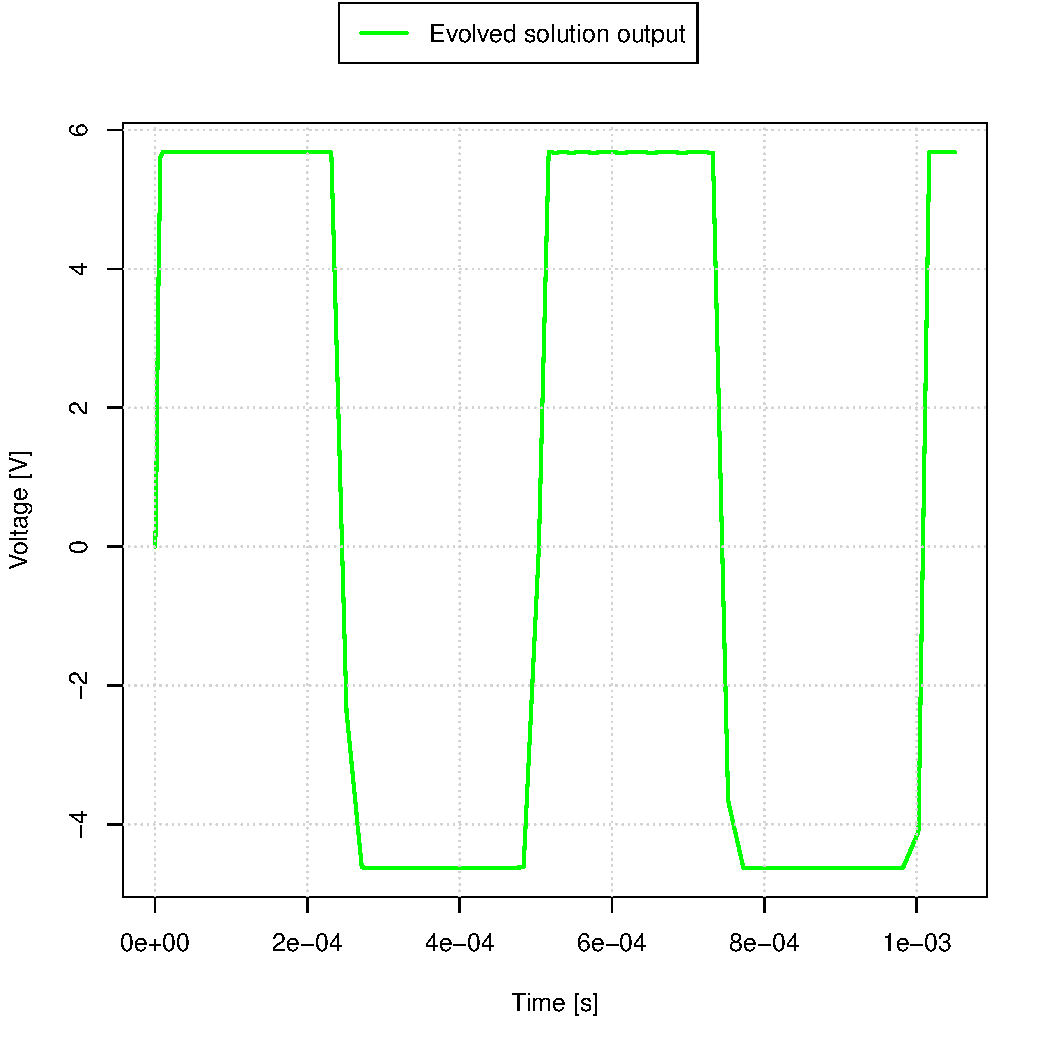
\includegraphics[scale=0.6]{best-solution-two-stage}\label{best-solution-two-stage-fig}}
    \caption{The best solution for the two stage amplifier found by the evolution}
\end{figure}

We can see that the resulting gain is approximately 50 (the amplitude of the input voltage is $Vin = \SI{100}{\milli\volt}$, the amplitude of the output voltage is approximately \SI{5}{\volt}, the supply voltage is $V1 = \SI{12}{\volt}$) but the output waveform is significantly distorted --- the circuit generates a square wave. The experiments did not provide any solution that would generate a sine wave. The components values for this solution are stated in table \ref{best-solution-two-stage-tab}.

\begin{table}[H]
\centering
\begin{tabular}{@{}cccccccccccccc@{}}
\toprule
    $R1$ [\si{\kilo\ohm}] & $R2$ [\si{\kilo\ohm}] & $Re$ [\si{\kilo\ohm}] & $Rc$ [\si{\kilo\ohm}] & $Ce$ [\si{\micro\farad}] & $Cin$ [\si{\micro\farad}] & $Cout$ [\si{\micro\farad}] \\
    $Rgb$ [\si{\ohm}] & $Reb$ [\si{\ohm}] & $Rcb$ [\si{\kilo\ohm}] & $R2b$ [\si{\kilo\ohm}] & $R1b$ [\si{\kilo\ohm}] & $Cm$ [\si{\micro\farad}] & $Ce2$ [\si{\micro\farad}] \\
    \midrule
    114 & 57  & 51.6 & 81.7 & 98   & 215 & 479 & \\
    22  & 298 & 3.37 & 9.24 & 80.5 & 351 & 139   \\
    \bottomrule
\end{tabular}
\caption{The best solution for the two stage amplifier found by the evolution}
\label{best-solution-two-stage-tab}
\end{table}

\chapter{Conclusion}
This thesis demonstrated the capabilities of the evolutionary algorithms, namely the evolution strategies, in the domain of the analog amplifiers design. In the first phase, the task was to implement the concept of evolution strategies and integrate it with the ngSPICE simulator. An inherent part of the evolutionary algorithms is an appropriate fitness function so the next step was to develop methods for evaluating the quality of the amplifiers. In the last stage, there were various experiments carried out in order to demonstrate the performance of the proposed solution.

There were two types of amplifiers chosen for the optimization and it emerged that the evolution has the capability to find the desired solution and that it can even provide different variations of a circuit that has the same amplification properties. However, the results for the second amplifier were considerably limited.

There were various types of the fitness function developed and evaluated during the implementation and users can choose the most appropriate one according to their needs. The results of experiments were also used for the determination of the most optimal parameters for the evolution. During the experiments, it also emerged that various extensions to the basic version of evolutionary strategies had a great influence on the overall performance of the algorithm.

The resulting application provides a tool for designing amplifiers with an arbitrary gain up to the maximum limits of the circuit without using any mathematical apparatus.

This thesis also contributed to the development of the ngSPICE simulator, which had memory leaks on various places in the source code. The simulator is run multiple times in a row during the optimization so there was a need to fix the memory leaks and the result is that they were successfully removed. The solution was proposed to the development team and the improvements will help in the next stages of development.

The future extension of this project could be an interface for entering various electronic circuits described in the SPICE syntax so that users could utilize the current implementation of evolution strategies with different fitness functions and they would not be limited only to the embedded circuits. % viz. obsah.tex / see obsah.tex

  % Pouzita literatura / Bibliography
  % ----------------------------------------------
\ifslovak
  \makeatletter
  \def\@openbib@code{\addcontentsline{toc}{chapter}{Literatúra}}
  \makeatother
  \bibliographystyle{bib-styles/czechiso}
\else
  \ifczech
    \makeatletter
    \def\@openbib@code{\addcontentsline{toc}{chapter}{Literatura}}
    \makeatother
    \bibliographystyle{bib-styles/czechiso}
  \else 
    \makeatletter
    \def\@openbib@code{\addcontentsline{toc}{chapter}{Bibliography}}
    \makeatother
    \bibliographystyle{bib-styles/englishiso}
  %  \bibliographystyle{alpha}
  \fi
\fi
  \begin{flushleft}
  \bibliography{thesis-20-literatura-bibliography}
  \end{flushleft}

  % vynechani stranky v oboustrannem rezimu
  % Skip the page in the two-sided mode
  \iftwoside
    \cleardoublepage
  \fi

  % Prilohy / Appendices
  % ---------------------------------------------
  \appendix
\ifczech
  \renewcommand{\appendixpagename}{Přílohy}
  \renewcommand{\appendixtocname}{Přílohy}
  \renewcommand{\appendixname}{Příloha}
\fi
\ifslovak
  \renewcommand{\appendixpagename}{Prílohy}
  \renewcommand{\appendixtocname}{Prílohy}
  \renewcommand{\appendixname}{Príloha}
\fi
  \appendixpage

% vynechani stranky v oboustrannem rezimu
% Skip the page in the two-sided mode
\iftwoside
  \cleardoublepage
\fi
  
\ifslovak
%  \section*{Zoznam príloh}
%  \addcontentsline{toc}{section}{Zoznam príloh}
\else
  \ifczech
%    \section*{Seznam příloh}
%    \addcontentsline{toc}{section}{Seznam příloh}
  \else
%    \section*{List of Appendices}
%    \addcontentsline{toc}{section}{List of Appendices}
  \fi
\fi
  \startcontents[chapters]
  % seznam příloh / list of appendices
  % \printcontents[chapters]{l}{0}{\setcounter{tocdepth}{2}}
  
  % vynechani stranky v oboustrannem rezimu
  \iftwoside
    \cleardoublepage
  \fi
  % Tento soubor nahraďte vlastním souborem s přílohami (nadpisy níže jsou pouze pro příklad)
% This file should be replaced with your file with an appendices (headings below are examples only)

% Umístění obsahu paměťového média do příloh je vhodné konzultovat s vedoucím
% Placing of table of contents of the memory media here should be consulted with a supervisor
%\chapter{Obsah přiloženého paměťového média}

%\chapter{Manuál}

%\chapter{Konfigurační soubor} % Configuration file

%\chapter{RelaxNG Schéma konfiguračního souboru} % Scheme of RelaxNG configuration file

%\chapter{Plakát} % poster

\chapter{User interface}
The program is implemented as a console application. The user can run the program in the following way:

\begin{verbatim}
bt [OPTIONS]...
\end{verbatim}

The \verb+OPTIONS+ are as follows:

\begin{description}[style=nextline]
    \item [\Q{-h, --help}] Prints the help message.

    \item [\Q{-o <directory_name>}] Specifies the output directory. By default, \Q{stdout} is used for the text output and the graphs are displayed on the screen.

    \item[\Q{--mu <number_of_ancestors>}] Sets the cardinality of the population of ancestors.\\
        The default value is 10 chromosomes.

    \item[\Q{--lambda <number_of_descendants>}] Sets the cardinality of the population of descendants.\\
        The default value is 150 chromosomes.

    \item[\Q{--max-gen <number_of_generations>}] Sets the maximum number of generations in the evolution.\\
        The default value is 3000 generations.

    \item[\Q{--stop-gen <number_of_generations>}] Sets the number of generations after which the terminating condition will be checked. This option is related to the \Q{stop-change} option.\\
        The default value is 500 generations.

    \item[\Q{--stop-change <value>}] The evolution terminates when the fitness of the best chromosome in the population does not decrease by a certain percentage after a certain number of generations. The percentage is set by this option. The value is in the interval $\left]0, 1\right]$.\\
        The default value is 0.99 meaning that the evolution terminates when the fitness does not change by more than 1\%.

    \item[\Q{--print-gen <number_of_generations>}] Sets the number of generations after which the print condition will be checked. This option is related to the \Q{print-change} option.\\
        The default value is 10 generations.

    \item[\Q{--print-change <value>}] The status of the evolution may be printed when the fitness of the best chromosome in the population decreases by a certain percentage after a certain number of generations. The percentage is set by this option. The value is in the interval ]0,1].\\
        The default value is 0.9 meaning that the status will be printed every time the fitness decreases by 10\%.

     \item[\Q{--ES (<'plus'> | <'comma'>)}] Specifies the selection scheme of the evolution strategies algorithm.\\
        The default value is \Q{'plus'}.

     \item[\Q{--max-res <maximum_resistance>}] Sets the maximum resistance of the circuit's resistors in ohms.\\
        The default value is \SI{200}{\kilo\ohm}.

     \item[\Q{--max-cap <maximum_capacitance>}] Sets the maximum capacitance of the circuit's capacitors in nanofarads.\\
        The default value is \SI{500}{\nano\farad}.

        \item[\Q{--sigma-init <initial_value>}] Sets the initial value of the mutation step.\\
        The default value is 100.

        \item[\Q{--fitness (<'bestMatch'> | <'idealSine'> | <'maxAmp'>)}] Specifies the evaluation method of the chromosomes' fitness.\\
        The default value is \Q{'bestMatch'}.

        \item[\Q{--amplitude <voltage>}] Sets the amplitude of the amplifier's output waveform in volts. This option only applies if the \Q{'idealSine'} evaluation method is used.\\
        The default value is \SI{1}{\volt}.

        \item[\Q{--Rload <resistance>}] Sets the resistance of the load resistor for the amplifier in ohms.\\
        The default value is \SI{22}{\kilo\ohm}.

        \item[\Q{--max-diff <difference>}] Sets the maximal percentage difference by which the trough and peak of the amplifier's output waveform may differ. The difference is in the interval ]0,100].\\
        The default value is 100\%.

        \item[\Q{--two-stage-amp}] Instead of the single stage amplifier, the subject of the optimization will be the two stage amplifier.
\end{description}

The output of the application contains graphs which were presented in the thesis and a text description which form is presented in listing \ref{evolution-output}. The description contains the values of all the optimized components of the two stage amplifier and their last mutation steps in the 270th generation. The print frequency may be set via \Q{OPTIONS}.

\begin{lstlisting}[caption={Evolution text output example},
                   label={evolution-output},
                   captionpos=b,
                   numbers=left]
Generation: 270
objective function: 22.7797
R1: 151 K, sigma: 1417.68
R2: 27.2 K, sigma: 49.2543
Re: 17.0 K, sigma: 0.920929
Rc: 40.2 K, sigma: 20.7433
Ce: 415 uF, sigma: 0.161956
Cin: 274 uF, sigma: 43.1271
Cout: 162 uF, sigma: 0.00136042
Rgb: 5.90 K, sigma: 75.8349
Reb: 17.8 K, sigma: 97.2993
Rcb: 10.4 K, sigma: 127.525
R2b: 185 K, sigma: 392.402
R1b: 200 K, sigma: 307.757
Cm: 159 uF, sigma: 261.11
Ce2: 184 uF, sigma: 73.005
\end{lstlisting}

You can stop the running application by sending the \Q{SIGQUIT} (\Q{Ctrl-\\}) signal. The \Q{SIGINT} signal does not work because the ngSPICE library uses it for its own purposes.

\chapter{CD content}
The attached CD contains

\begin{itemize}
    \item the modified source code of ngSPICE,
    \item the implementation of the evolutionary algorithms in C++,
    \item shell scripts for performing experiments with both the single and two stage amplifiers,
    \item the electronic version of this document along with its source code in \LaTeX,
    \item file \Q{README.txt} which describes the compilation of the application and other auxiliary files.
\end{itemize}

\chapter{Jak pracovat s touto šablonou}
\label{jak}

V této kapitole je uveden popis jednotlivých částí šablony, po kterém následuje stručný návod, jak s touto šablonou pracovat. 

Jedná se o přechodnou verzi šablony. Nová verze bude zveřejněna do konce roku 2016 a bude navíc obsahovat nové pokyny ke správnému využití šablony, závazné pokyny k~vypracování bakalářských a diplomových prací (rekapitulace pokynů, které jsou dostupné na~webu) a nezávazná doporučení od vybraných vedoucích. Jediné soubory, které se v nové verzi změní, budou projekt-01-kapitoly-chapters.tex a projekt-30-prilohy-appendices.tex, jejichž obsah každý student vymaže a nahradí vlastním. Šablonu lze tedy bez problémů využít i~v~současné verzi.

\section*{Popis částí šablony}

Po rozbalení šablony naleznete následující soubory a adresáře:
\begin{DESCRIPTION}
  \item [bib-styles] Styly literatury (viz níže). 
  \item [obrazky-figures] Adresář pro Vaše obrázky. Nyní obsahuje placeholder.pdf (tzv. TODO obrázek, který lze použít jako pomůcku při tvorbě technické zprávy), který se s prací neodevzdává. Název adresáře je vhodné zkrátit, aby byl jen ve zvoleném jazyce.
  \item [template-fig] Obrázky šablony (znak VUT).
  \item [fitthesis.cls] Šablona (definice vzhledu).
  \item [Makefile] Makefile pro překlad, počítání normostran, sbalení apod. (viz níže).
  \item [projekt-01-kapitoly-chapters.tex] Soubor pro Váš text (obsah nahraďte).
  \item [projekt-20-literatura-bibliography.bib] Seznam literatury (viz níže).
  \item [projekt-30-prilohy-appendices.tex] Soubor pro přílohy (obsah nahraďte).
  \item [projekt.tex] Hlavní soubor práce -- definice formálních částí.
\end{DESCRIPTION}

Výchozí styl literatury (czechiso) je od Ing. Martínka, přičemž anglická verze (englishiso) je jeho překladem s drobnými modifikacemi. Oproti normě jsou v něm určité odlišnosti, ale na FIT je dlouhodobě akceptován. Alternativně můžete využít styl od Ing. Radima Loskota nebo od Ing. Radka Pyšného\footnote{BP Ing. Radka Pyšného \url{http://www.fit.vutbr.cz/study/DP/BP.php?id=7848}}. Alternativní styly obsahují určitá vylepšení, ale zatím nebyly řádně otestovány větším množstvím uživatelů. Lze je považovat za beta verze pro zájemce, kteří svoji práci chtějí mít dokonalou do detailů a neváhají si nastudovat detaily správného formátování citací, aby si mohli ověřit, že je vysázený výsledek v pořádku.

Makefile kromě překladu do PDF nabízí i další funkce:
\begin{itemize}
  \item přejmenování souborů (viz níže),
  \item počítání normostran,
  \item spuštění vlny pro doplnění nezlomitelných mezer,
  \item sbalení výsledku pro odeslání vedoucímu ke kontrole (zkontrolujte, zda sbalí všechny Vámi přidané soubory, a případně doplňte).
\end{itemize}

Nezapomeňte, že vlna neřeší všechny nezlomitelné mezery. Vždy je třeba manuální kontrola, zda na konci řádku nezůstalo něco nevhodného -- viz Internetová jazyková příručka\footnote{Internetová jazyková příručka \url{http://prirucka.ujc.cas.cz/?id=880}}.

\paragraph {Pozor na číslování stránek!} Pokud má obsah 2 strany a na 2. jsou jen \uv{Přílohy} a~\uv{Seznam příloh} (ale žádná příloha tam není), z nějakého důvodu se posune číslování stránek o 1 (obsah \uv{nesedí}). Stejný efekt má, když je na 2. či 3. stránce obsahu jen \uv{Literatura} a~je možné, že tohoto problému lze dosáhnout i jinak. Řešení je několik (od~úpravy obsahu, přes nastavení počítadla až po sofistikovanější metody). \textbf{Před odevzdáním proto vždy překontrolujte číslování stran!}


\section*{Doporučený postup práce se šablonou}

\begin{enumerate}
  \item \textbf{Zkontrolujte, zda máte aktuální verzi šablony.} Máte-li šablonu z předchozího roku, na stránkách fakulty již může být novější verze šablony s~aktualizovanými informacemi, opravenými chybami apod.
  \item \textbf{Zvolte si jazyk}, ve kterém budete psát svoji technickou zprávu (česky, slovensky nebo anglicky) a svoji volbu konzultujte s vedoucím práce (nebyla-li dohodnuta předem). Pokud Vámi zvoleným jazykem technické zprávy není čeština, nastavte příslušný parametr šablony v souboru projekt.tex (např.: \verb|documentclass[english]{fitthesis}| a přeložte prohlášení a poděkování do~angličtiny či slovenštiny.
  \item \textbf{Přejmenujte soubory.} Po rozbalení je v šabloně soubor projekt.tex. Pokud jej přeložíte, vznikne PDF s technickou zprávou pojmenované projekt.pdf. Když vedoucímu více studentů pošle projekt.pdf ke kontrole, musí je pracně přejmenovávat. Proto je vždy vhodné tento soubor přejmenovat tak, aby obsahoval Váš login a (případně zkrácené) téma práce. Vyhněte se však použití mezer, diakritiky a speciálních znaků. Vhodný název tedy může být např.: \uv{xlogin00-Cisteni-a-extrakce-textu.tex}. K přejmenování můžete využít i přiložený Makefile:
\begin{verbatim}
make rename NAME=xlogin00-Cisteni-a-extrakce-textu
\end{verbatim}
  \item Vyplňte požadované položky v souboru, který byl původně pojmenován projekt.tex, tedy typ, rok (odevzdání), název práce, svoje jméno, ústav (dle zadání), tituly a~jméno vedoucího, abstrakt, klíčová slova a další formální náležitosti.
  \item Nahraďte obsah souborů s kapitolami práce, literaturou a přílohami obsahem svojí technické zprávy. Jednotlivé přílohy či kapitoly práce může být výhodné uložit do~samostatných souborů -- rozhodnete-li se pro toto řešení, je doporučeno zachovat konvenci pro názvy souborů, přičemž za číslem bude následovat název kapitoly. 
  \item Nepotřebujete-li přílohy, zakomentujte příslušnou část v projekt.tex a příslušný soubor vyprázdněte či smažte. Nesnažte se prosím vymyslet nějakou neúčelnou přílohu jen proto, aby daný soubor bylo čím naplnit. Vhodnou přílohou může být obsah přiloženého paměťového média.
  \item Nascanované zadání uložte do souboru zadani.pdf a povolte jeho vložení do práce parametrem šablony v projekt.tex (\verb|documentclass[zadani]{fitthesis}|).
  \item Nechcete-li odkazy tisknout barevně (tedy červený obsah -- bez konzultace s vedoucím nedoporučuji), budete pro tisk vytvářet druhé PDF s tím, že nastavíte parametr šablony pro tisk: (\verb|documentclass[zadani,print]{fitthesis}|).  Barevné logo se nesmí tisknout černobíle!
  \item Vzor desek, do kterých bude práce vyvázána, si vygenerujte v informačním systému fakulty u zadání. Pro disertační práci lze zapnout parametrem v šabloně (více naleznete v souboru fitthesis.cls).
  \item Nezapomeňte, že zdrojové soubory i (obě verze) PDF musíte odevzdat na CD či jiném médiu přiloženém k technické zprávě.
\end{enumerate}

\subsection*{Pokyny pro oboustranný tisk}
\begin{itemize}
\item Zapíná se parametrem šablony: \verb|\documentclass[twoside]{fitthesis}|
\item Po vytištění oboustranného listu zkontrolujte, zda je při prosvícení sazební obrazec na obou stranách na stejné pozici. Méně kvalitní tiskárny s duplexní jednotkou mají často posun o 1--3 mm. Toto může být u některých tiskáren řešitelné tak, že vytisknete nejprve liché stránky, pak je dáte do stejného zásobníku a vytisknete sudé.
\item Za titulním listem, obsahem, literaturou, úvodním listem příloh, seznamem příloh a případnými dalšími seznamy je třeba nechat volnou stránku, aby následující část začínala na liché stránce (\textbackslash cleardoublepage).
\item  Konečný výsledek je nutné pečlivě překontrolovat.
\end{itemize}


\subsection*{Užitečné nástroje}
\label{nastroje}

Následující seznam není výčtem všech využitelných nástrojů. Máte-li vyzkoušený osvědčený nástroj, neváhejte jej využít. Pokud však nevíte, který nástroj si zvolit, můžete zvážit některý z následujících:

\begin{description}
	\item[\href{http://miktex.org/download}{MikTeX}] \LaTeX{} pro Windows -- distribuce s jednoduchou instalací a vynikající automatizací stahování balíčků.
	\item[\href{http://texstudio.sourceforge.net/}{TeXstudio}] Přenositelné opensource GUI pro \LaTeX{}.  Ctrl+klik umožňuje přepínat mezi zdrojovým textem a PDF. Má integrovanou kontrolu pravopisu, zvýraznění syntaxe apod. Pro jeho využití je nejprve potřeba nainstalovat MikTeX.
	\item[\href{http://jabref.sourceforge.net/download.php}{JabRef}] Pěkný a jednoduchý program v Javě pro správu souborů s bibliografií (literaturou). Není potřeba se nic učit -- poskytuje jednoduché okno a formulář pro editaci položek.
	\item[\href{https://inkscape.org/en/download/}{InkScape}] Přenositelný opensource editor vektorové grafiky (SVG i PDF). Vynikající nástroj pro tvorbu obrázků do odborného textu. Jeho ovládnutí je obtížnější, ale výsledky stojí za to.
	\item[\href{https://git-scm.com/}{GIT}] Vynikající pro týmovou spolupráci na projektech, ale může výrazně pomoci i jednomu autorovi. Umožňuje jednoduché verzování, zálohování a přenášení mezi více počítači.
	\item[\href{http://www.overleaf.com/}{Overleaf}] Online nástroj pro \LaTeX{}. Přímo zobrazuje náhled a umožňuje jednoduchou spolupráci (vedoucí může průběžně sledovat psaní práce), vyhledávání ve zdrojovém textu kliknutím do PDF, kontrolu pravopisu apod. Zdarma jej však lze využít pouze s určitými omezeními (někomu stačí na disertaci, jiný na ně může narazit i při psaní bakalářské práce) a pro dlouhé texty je pomalejší.
\end{description}

\subsection*{Užitečné balíčky pro \LaTeX}

Studenti při sazbě textu často řeší stejné problémy. Některé z nich lze vyřešit následujícími balíčky pro \LaTeX:

\begin{itemize}
  \item \verb|amsmath| -- rozšířené možnosti sazby rovnic,
  \item \verb|float, afterpage, placeins| -- úprava umístění obrázků,
  \item \verb|fancyvrb, alltt| -- úpravy vlastností prostředí Verbatim, 
  \item \verb|makecell| -- rozšíření možností tabulek,
  \item \verb|pdflscape, rotating| -- natočení stránky o 90 stupňů (pro obrázek či tabulku),
  \item \verb|hyphenat| -- úpravy dělení slov,
  \item \verb|picture, epic, eepic| -- přímé kreslení obrázků.
\end{itemize}

Některé balíčky jsou využity přímo v šabloně (v dolní části souboru fitthesis.cls). Nahlédnutí do jejich dokumentace může být rovněž užitečné.

Sloupec tabulky zarovnaný vlevo s pevnou šířkou je v šabloně definovaný \uv{L} (používá se jako \uv{p}).

 % viz. prilohy.tex / see prilohy.tex
\end{document}
